\documentclass[12pt,a4paper]{extarticle}

\usepackage[a4paper, left=2.5cm, right=1.5cm, top=1.5cm, bottom=1.5cm]{geometry}
\usepackage{fontspec}
\setmainfont{Times New Roman}[
  Ligatures=TeX,
  BoldFont = * Bold,
  ItalicFont = * Italic,
  BoldItalicFont = * Bold Italic,
]
\usepackage[ukrainian]{babel}
\usepackage{graphicx}
\graphicspath{ {./images/} }
\usepackage{caption}
\usepackage{amsmath}
\usepackage{amssymb}
\usepackage{setspace}
\usepackage{microtype}
\usepackage{ragged2e}
\usepackage{etoolbox}
\usepackage{fancyhdr}
\usepackage{indentfirst}

\setlength{\headheight}{17pt}

\setstretch{1.25}
\justifying
\setlength{\parindent}{7mm}
\setlength{\parskip}{0pt}

\addto\captionsukrainian{%
  \renewcommand{\figurename}{Рис.}%
  \renewcommand{\contentsname}{Зміст}%
  \def\partname{Розділ}%
}
\renewcommand{\thepart}{\arabic{part}}
\numberwithin{section}{part}
\setcounter{secnumdepth}{2}
\setcounter{tocdepth}{2}

\pagestyle{fancy}
\fancyhf{}
\fancyhead[C]{\thepage}
\renewcommand{\headrulewidth}{0pt}
\fancypagestyle{plain}{%
  \fancyhf{}%
  \fancyhead[C]{\thepage}%
  \renewcommand{\headrulewidth}{0pt}%
}

\makeatletter
\renewcommand\tableofcontents{%
  \clearpage
  \begin{center}
    {\large\bfseries\MakeUppercase{\contentsname}}
  \end{center}
  \vspace{0.8em}
  \begingroup
    \singlespacing
    \RaggedRight
    \setlength{\parindent}{0pt}%
    \setlength{\parskip}{0pt}%
    \@starttoc{toc}%
  \endgroup
}
\makeatother

\usepackage[hidelinks, unicode=true]{hyperref}
\hypersetup{
  pdftitle={Словничок термінів з математичної нелінійної оптимізації},
  pdfauthor={Кіщук Ярослав},
  pdfsubject={Негладкий аналіз та оптимізація},
  pdfkeywords={негладкий аналіз, оптимізація, субдиференціал, квазідиференціал, кодиференціал},
}

\makeatletter
\def\@part[#1]#2{%
    \ifnum \c@secnumdepth >\m@ne
      \refstepcounter{part}%
      \addcontentsline{toc}{part}{\protect\numberline{\thepart}#1}%
    \else
      \addcontentsline{toc}{part}{#1}%
    \fi
    {\parindent \z@ \raggedright
     \interlinepenalty \@M
     \normalfont
     \ifnum \c@secnumdepth >\m@ne
       \Large\bfseries \partname~\thepart
       \par\nobreak
     \fi
     \huge \bfseries #2%
     \markboth{}{}\par}%
    \nobreak
    \vskip 3ex
    \@afterheading}
\renewcommand*{\l@part}[2]{%
  \addpenalty{-\@highpenalty}%
  \addvspace{0.8em \@plus\p@}%
  \begingroup
    \bfseries
    \@dottedtocline{0}{0em}{2.5em}{#1}{#2}%
  \endgroup
}
\renewcommand*{\l@section}{\@dottedtocline{1}{0em}{2.8em}}
\makeatother

\begin{document}

\begin{titlepage}
\thispagestyle{empty}
\begin{center}
\vspace*{3cm}
{\Large\bfseries Словничок термінів та основних понять\\[0.3em] з математичної нелінійної оптимізації}\\[1.2cm]
{\normalsize на основі матеріалу лекцій Джалладової І.~А.\\ та посібника М.~П.~Моклячука\\[0.2em] \emph{«Негладкий аналіз та оптимізація»}}\\[2cm]
{\large Виконав: Кіщук Ярослав}\\[0.4cm]
{\normalsize Викладач: Джалладова І.~А.}
\vfill
{\normalsize Київ~--- 2026}
\end{center}
\end{titlepage}

\tableofcontents
\clearpage
\part{Опуклі множини}

\section{Опукла множина.}
Непорожню множину $X \subset \mathbb{R}^{n}$ називають опуклою, якщо для будь-яких двох її точок уся точка відрізка між ними також належить $X$:

$$
x_{1}, x_{2} \in X, \quad 0 \leq \lambda \leq 1 \quad \Longrightarrow \quad \lambda x_{1}+(1-\lambda) x_{2} \in X .
$$

\section{Афінна множина.}
Множину $X \subset \mathbb{R}^{n}$ називають афінною, якщо разом із двома довільними точками вона містить усю пряму, що їх з’єднує:

$$
x_{1}, x_{2} \in X, \quad \lambda \in \mathbb{R} \quad \Longrightarrow \quad \lambda x_{1}+(1-\lambda) x_{2} \in X .
$$

\section{Конус і опуклий конус.}
Множину $K \subset \mathbb{R}^{n}$ називають конусом, якщо з умови $x \in K$ випливає $\lambda x \in K$ для всіх $\lambda>0$. Опуклий конус замкнений щодо додавання та множення на додатні числа:

$$
x_{1}, x_{2} \in K, \quad \lambda_{1}, \lambda_{2}>0 \quad \Longrightarrow \quad \lambda_{1} x_{1}+\lambda_{2} x_{2} \in K .
$$

\section{Опукла, конічна, афінна і лінійна комбінації.}
Лінійну комбінацію точок $x_{1}, \ldots, x_{m}$ записують як $\sum_{i=1}^{m} \lambda_{i} x_{i}$. Залежно від обмежень на коефіцієнти $\lambda_i$ розрізняють такі типи:

$$
\begin{array}{ll}
\text { опуклою, якщо } & \lambda_{i} \geq 0, \quad \sum_{i} \lambda_{i}=1, \\
\text { конічною, якщо } & \lambda_{i} \geq 0, \\
\text { афінною, якщо } & \sum_{i} \lambda_{i}=1, \\
\text { лінійною, якщо } & \lambda_{i} \in \mathbb{R}^{1} .
\end{array}
$$

\section{Оболонка точок: опукла, конічна, афінна, лінійна.}
Використовуються такі позначення (у порядку: опукла, конічна, афінна, лінійна):

$$
\operatorname{conv} X, \quad \operatorname{cone} X, \quad \operatorname{aff} X, \quad \operatorname{Lin} X .
$$

Перетин усіх опуклих (відповідно: конічних, афінних, лінійних) множин, що містять $X$, називають опуклою (конічною, афінною, лінійною) оболонкою множини $X$.

\section{Відносне нутро множини.}
Багато опуклих множин у $\mathbb{R}^n$ --- наприклад, відрізок у $\mathbb{R}^2$ або плоский многогранник у $\mathbb{R}^3$ --- не мають внутрішності в звичайному топологічному сенсі ($\operatorname{int} X = \emptyset$). Для коректного аналізу таких множин застосовують поняття відносного нутра.

\textbf{Означення.} \textit{Відносним нутром} опуклої множини $X \subset \mathbb{R}^n$ (позначення $\operatorname{ri} X$) називають множину точок, які є внутрішніми відносно афінної оболонки $\operatorname{aff} X$:
$$
\operatorname{ri} X = \{ x \in X \mid \exists \varepsilon > 0 : B(x, \varepsilon) \cap \operatorname{aff} X \subset X \},
$$
де $B(x, \varepsilon) = \{ y \in \mathbb{R}^n \mid \|y - x\| < \varepsilon \}$ --- відкрита куля радіуса $\varepsilon$ із центром у точці $x$.

\textbf{Основні властивості відносного нутра:}
\begin{enumerate}
    \item Для непорожньої опуклої множини $X$ відносне нутро непорожнє: $\operatorname{ri} X \neq \emptyset$.
    \item Замикання відносного нутра збігається із замиканням множини: $\overline{\operatorname{ri} X} = \overline{X}$.
    \item Операція взяття відносного нутра ідемпотентна: $\operatorname{ri}(\operatorname{ri} X) = \operatorname{ri} X$.
    \item Якщо $x \in \operatorname{ri} X$ і $y \in \overline{X}$, то для кожного $\lambda \in (0, 1]$ маємо $\lambda x + (1-\lambda)y \in \operatorname{ri} X$.
\end{enumerate}

\begin{figure}[htbp]
\centering
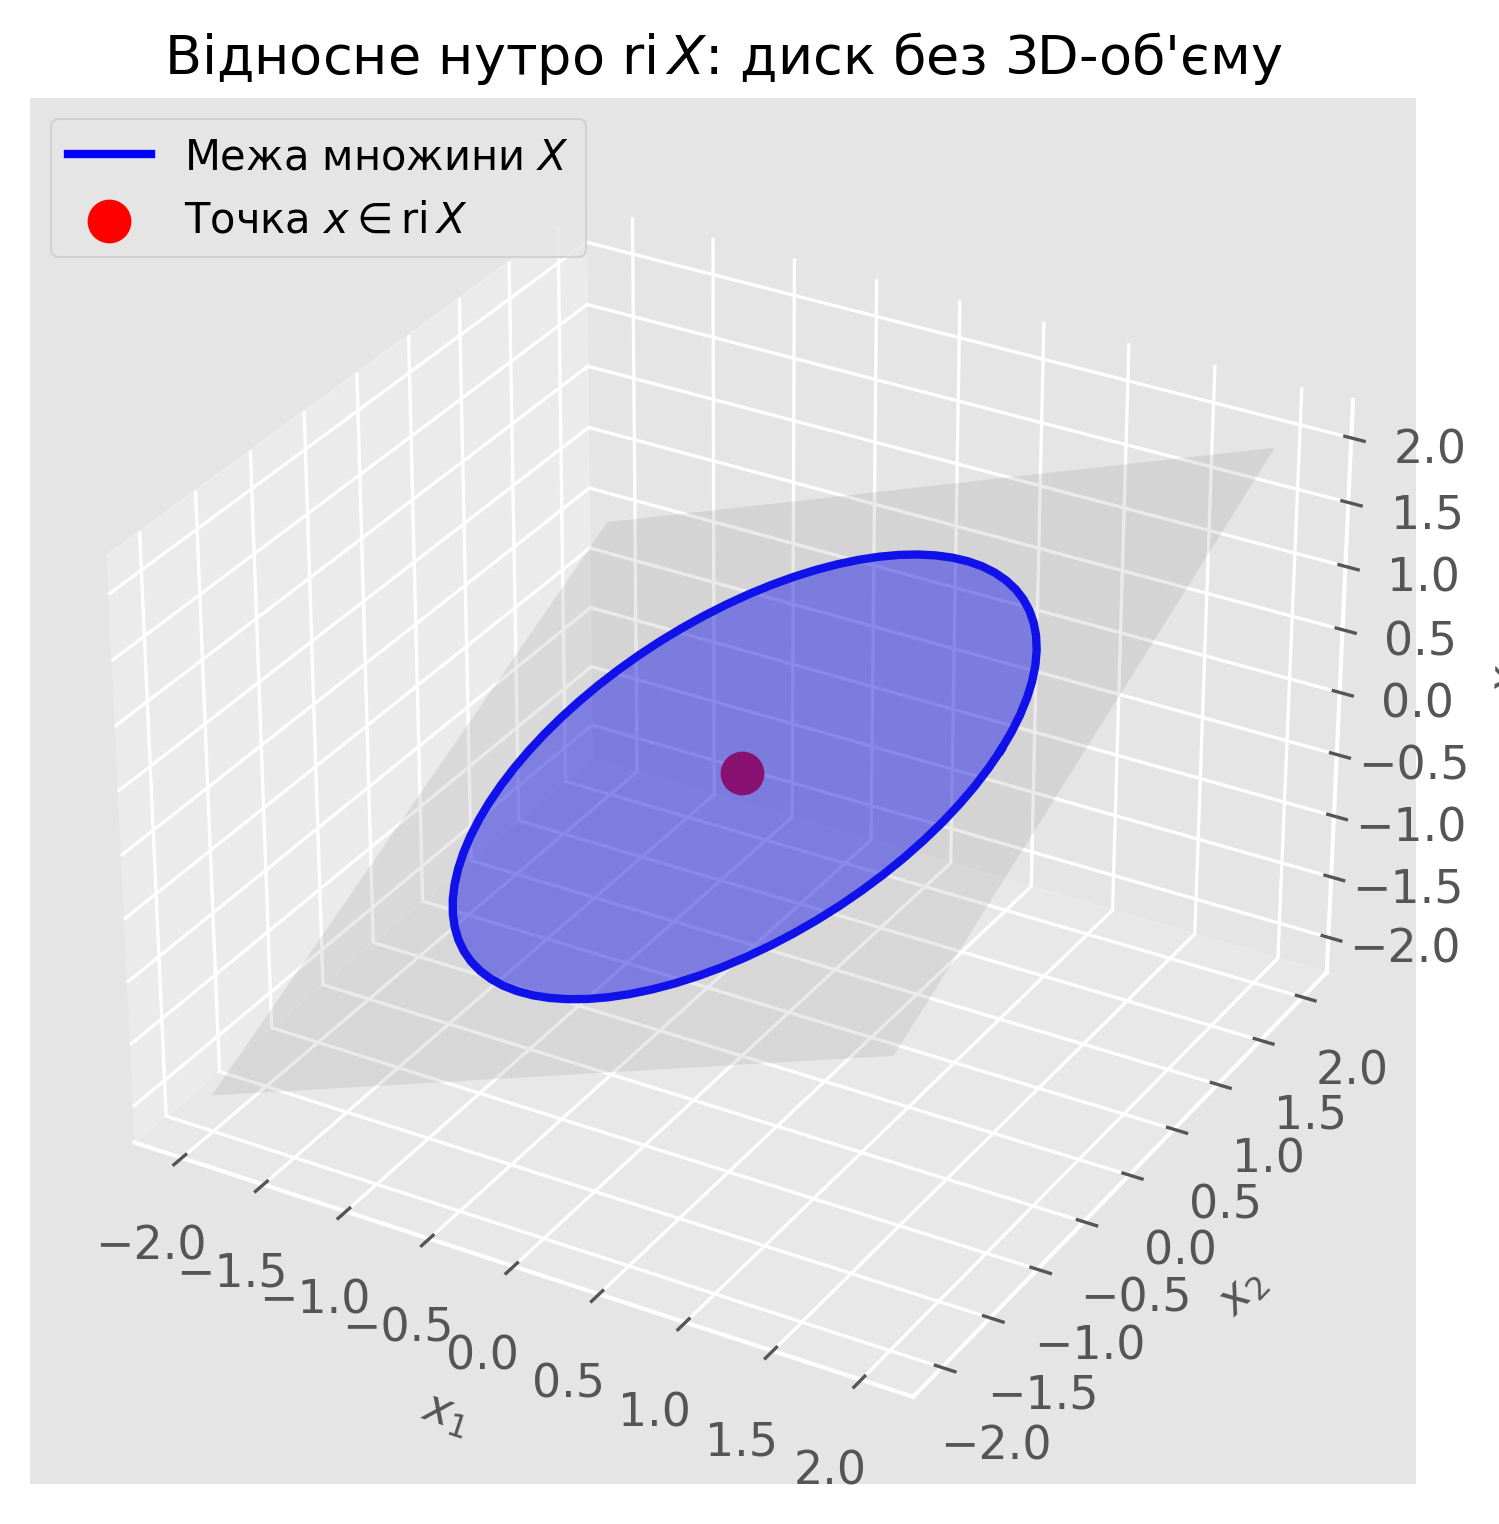
\includegraphics[width=0.85\textwidth]{relative_interior.png}
\caption{Геометричний зміст відносного нутра: диск не має об'єму у 3D просторі (звичайне нутро порожнє), але має внутрішність відносно своєї афінної площини.}
\label{fig:relative-interior}
\end{figure}

\section{Підпростір, гіперплощина, півпростір, промінь.}
Гіперплощину з нормаллю $p$ задають рівнянням

$$
H_{p \beta}=\left\{x \in \mathbb{R}^{n}:\langle p, x\rangle=\beta\right\} .
$$

Їй відповідають два півпростори:

$$
H_{p \beta}^{+}=\{x:\langle p, x\rangle \geq \beta\}, \quad H_{p \beta}^{-}=\{x:\langle p, x\rangle \leq \beta\} .
$$

Промінь із точки $\widehat{x}$ у напрямку $h$ має вигляд

$$
\ell_{\widehat{x} h}^{+}=\{\widehat{x}+\alpha h: \alpha \geq 0\} .
$$

\section{Поліедр, многогранні множини, многогранний конус.}
Поліедри та многогранні множини описують скінченними системами лінійних нерівностей.\\
\textit{Поліедром} називають множину розв'язків скінченної системи лінійних нерівностей, тобто перетин скінченної кількості півпросторів:

$$
X=\left\{x \in \mathbb{R}^{n}:\left\langle a^{i}, x\right\rangle \leq b_{i}, і \in I=\{1, \ldots, m\}\right\},
$$

або

$$
X=\left\{x \in \mathbb{R}^{n}: A x \leq b\right\},
$$

де $b=\left(b_{1}, \ldots, b_{m}\right) \in \mathbb{R}^{m}, A$ --- матриця розмірності $m \times n$ з рядками $a^{1}, a^{2}, \ldots, a^{m} \in \mathbb{R}^{n}$.\\
\textit{Опуклим многогранником} називають опуклу оболонку скінченної множини точок; кожен такий многогранник можна також задати скінченною системою лінійних нерівностей, і навпаки --- будь-який обмежений поліедр є опуклим многогранником.

Опуклий многогранник $X=\operatorname{conv}\left\{x^{1}, \ldots, x^{m}\right\}$ має параметричний опис

$$
X=\left\{x \in \mathbb{R}^{n} \mid x=\sum_{i=1}^{m} \lambda_{i} x^{i}, \lambda_{i} \geq 0 ; \sum_{i=1}^{m} \lambda_{i}=1\right\} .
$$

Опорна функція многогранника має вигляд

$$
s\left(x^{*} \mid M\right)=\sup _{x \in M}\left\langle x, x^{*}\right\rangle=\max _{1 \leq і \leq m}\left\langle x^{i}, x^{*}\right\rangle
$$

Нехай

$$
I\left(x^{*}\right)=\left\{i:\left\langle x^{i}, x^{*}\right\rangle=s\left(x^{*} \mid M\right), i=1, \ldots, m\right\}
$$

тобто $I\left(x^{*}\right)$ --- множина індексів $i$, для яких скалярний добуток $\left\langle x^{i}, x^{*}\right\rangle$ набуває максимального значення.

Гіперплощина

$$
\left\{x:\left\langle x, x^{*}\right\rangle=s\left(x^{*} \mid M\right)\right\}
$$

називають \textit{опорною гіперплощиною}. Якщо $j \in I\left(x^{*}\right)$ і серед векторів $\left\langle x^{i}-x^{j}, x^{*}\right\rangle=0$, $i \in I\left(x^{*}\right)$ знайдеться $n$ лінійно незалежних, опору називають \textit{крайньою}.

\textit{Многогранною множиною} називають множину точок, що задовольняють систему лінійних нерівностей

$$
\left\langle x, x_{i}^{*}\right\rangle \geq \alpha_{i}, \quad i=1, \ldots, l
$$

\textit{Многогранним конусом} називають конус $K$, для якого існує скінченний набір векторів $x_{1}, \ldots, x_{m}$ такий, що кожен $x \in K$ (і лише такий $x$) подається у вигляді

$$
x=\sum_{i=1}^{m} \lambda_{i} x_{i}, \quad \lambda_{i} \geq 0, \quad i=1, \ldots, m
$$

Многогранний конус також можна задати скінченною системою лінійних однорідних нерівностей

$$
\left\langle x, x_{k}^{*}\right\rangle \geq 0, \quad k=1, \ldots, l
$$

% ==========================================
% ДОДАТКОВІ СЕКЦІЇ ДО РОЗДІЛУ 1 (ОПУКЛІ МНОЖИНИ)
% ==========================================

\section{Крайня точка.}
Точку $x$ опуклої множини $X$ називають \textit{крайньою}, якщо з подання

$$
x=\lambda x_{1}+(1-\lambda) x_{2}, \quad 0<\lambda<1, \quad x_{1}, x_{2} \in X,
$$

випливає $x_{1}=x_{2}=x$.\\
\textit{Критерій існування крайньої точки:} нехай $X$ --- замкнута опукла множина в $\mathbb{R}^{n}$. Тоді $X$ містить принаймні одну крайню точку тоді і лише тоді, коли в $X$ не вкладено жодної прямої, тобто множини виду

$$
l_{x^{0} h}=\left\{x \in \mathbb{R}^{n}: x=x^{0}+\alpha h, \alpha \in \mathbb{R}\right\},
$$

де $x^{0} \in \mathbb{R}^{n}, h \in \mathbb{R}^{n}, h \neq 0$.

\section{Теорема Радона.}
Теорема Радона описує комбінаторні властивості опуклих оболонок скінченних систем точок у скінченновимірних просторах.

\textbf{Теорема (Радона).} Будь-яку множину $S \subset \mathbb{R}^n$ із щонайменше $n + 2$ точок можна розбити на дві неперетні підмножини $S_1$ та $S_2$ ($S = S_1 \cup S_2$, $S_1 \cap S_2 = \emptyset$) так, що їхні опуклі оболонки перетинаються:
$$
\operatorname{conv} S_1 \cap \operatorname{conv} S_2 \neq \emptyset.
$$

\section{Теорема Хеллі.}
Теорема Хеллі дає умови, за яких перетин усієї родини опуклих множин непорожній, якщо непорожні перетини всіх скінченних підсистем достатнього розміру.

\textbf{Теорема (Хеллі).} Нехай $\{X_i\}_{i \in I}$ --- скінченна родина опуклих множин у $\mathbb{R}^n$, що містить щонайменше $n + 1$ елемент. Якщо будь-які $n + 1$ множини цієї родини мають непорожній перетин, то й перетин усієї родини непорожній:
$$
\bigcap_{i \in I} X_i \neq \emptyset.
$$
\textit{Зауваження:} твердження залишається в силі й для нескінченної родини опуклих множин за додаткової умови компактності (хоча б одна множина або всі множини --- замкнені й обмежені).

\section{Теорема Каратеодорі.}
Нехай $\operatorname{dim} \operatorname{Lin} X=n$. Будь-яку точку опуклої, конічної, афінної або лінійної оболонки множини $X$ можна представити як відповідну комбінацію не більш ніж $r$ точок $x^{1}, \ldots, x^{r}$ з $X$. Для опуклої та афінної оболонок $r=n+1$, причому ці точки можна обрати афінно незалежними. Для конічної та лінійної оболонок $r=n$, причому ці точки можна обрати лінійно незалежними.

\section{Теорема про розділення множин.}
Ідея теорем розділення полягає в тому, що неперетинні опуклі множини за певних умов можна відділити ненульовим лінійним функціоналом. Нижче наведено основні формулювання.\\
Теорема 1.4.1. Нехай $M$ --- опукла множина і $x_{0} \notin \bar{M}$. Тоді існують $x^{*} \neq 0$ та $\varepsilon>0$ такі, що

$$
\left\langle x, x^{*}\right\rangle \leq\left\langle x_{0}, x^{*}\right\rangle-\varepsilon
$$

для всіх $x \in M$.\\
Теорема 1.4.2. Нехай $M$ --- опукла множина і точка $x_{0} \notin M$. Тоді існує $x^{*} \neq 0$, що задовольняє нерівності

$$
\left\langle x, x^{*}\right\rangle \leq\left\langle x_{0}, x^{*}\right\rangle
$$

для всіх $x \in M$.\\
Теорема 1.4.3. Нехай $M_{1}, M_{2}$ --- опуклі множини, що не перетинаються. Тоді існує така точка $x^{*} \neq 0$, що виконується нерівність

$$
\left\langle x_{1}, x^{*}\right\rangle \leq\left\langle x_{2}, x^{*}\right\rangle
$$

для всіх $x_{1} \in M_{1}, x_{2} \in M_{2}$.\\
Теорема 1.4.4. Нехай $M_{1}, M_{2}$ --- замкнуті опуклі множини, що не перетинаються. Нехай одна з множин компактна. Тоді існує точка $x^{*}$ і число $\varepsilon>0$ такі, що

$$
\left\langle x_{1}, x^{*}\right\rangle \leq\left\langle x_{2}, x^{*}\right\rangle-\varepsilon
$$

для всіх $x_{1} \in M_{1}, x_{2} \in M_{2}$.\\
Теорема 1.4.5. Нехай $M$ --- замкнута опукла множина. Тоді $x \in M$ тоді і тільки тоді, коли

$$
\left\langle x, x^{*}\right\rangle \leq s\left(x^{*} \mid M\right)
$$

для всіх $x^{*} \in M$.

\section{Теорема Мінковського про опуклий компакт.}
Якщо $X$ --- опуклий компакт у $\mathbb{R}^{n}$, то він є опуклою оболонкою множини своїх крайніх точок: $X=\operatorname{conv} E(X)$, де $E(X)$ --- множина крайніх точок $X$.

\section{Проекція точки на опуклу множину та варіаційна нерівність.}
\textbf{Означення.} Нехай $X \subset \mathbb{R}^n$ --- замкнена опукла множина, а $y \in \mathbb{R}^n$ --- довільна точка. \textit{Проекцією} точки $y$ на $X$ (позначення $P_X(y)$) називають точку $X$ з мінімальною відстанню до $y$:
$$
P_X(y) = \arg\min_{x \in X} \|x - y\|.
$$

Завдяки строгій опуклості евклідової норми та замкненості множини $X$, проекція існує і є єдиною для будь-якої точки $y \in \mathbb{R}^n$.

\textbf{Теорема (Характеристична властивість проекції / Варіаційна нерівність).} Точка $z \in X$ є проекцією точки $y$ на замкнену опуклу множину $X$ ($z = P_X(y)$) тоді і тільки тоді, коли виконується варіаційна нерівність:
$$
\langle y - z, x - z \rangle \leq 0 \quad \forall x \in X.
$$

Геометрично: кут між вектором зсуву $y - P_X(y)$ та будь-яким вектором $x - P_X(y)$, спрямованим всередину множини $X$, є тупим або прямим.

\section{Спряжений конус і поляра конуса.}
Для конуса $K$ поляра має вигляд

$$
K^{0}=\left\{x^{*} \in X^{*}:\left\langle x^{*}, x\right\rangle \leq 0, \forall x \in K\right\} .
$$

Спряжений конус вводять як

$$
K^{*}=-K^{0} .
$$

\section{Функція Мінковського.}
Для множини $A \subset X$ функція Мінковського задається формулою

$$
\mu(x \mid A)= \begin{cases}0, & x=0 \\ \inf \left\{\lambda>0: \lambda^{-1} x \in A\right\}, & x \neq 0\end{cases}
$$

\begin{figure}[htbp]
\centering
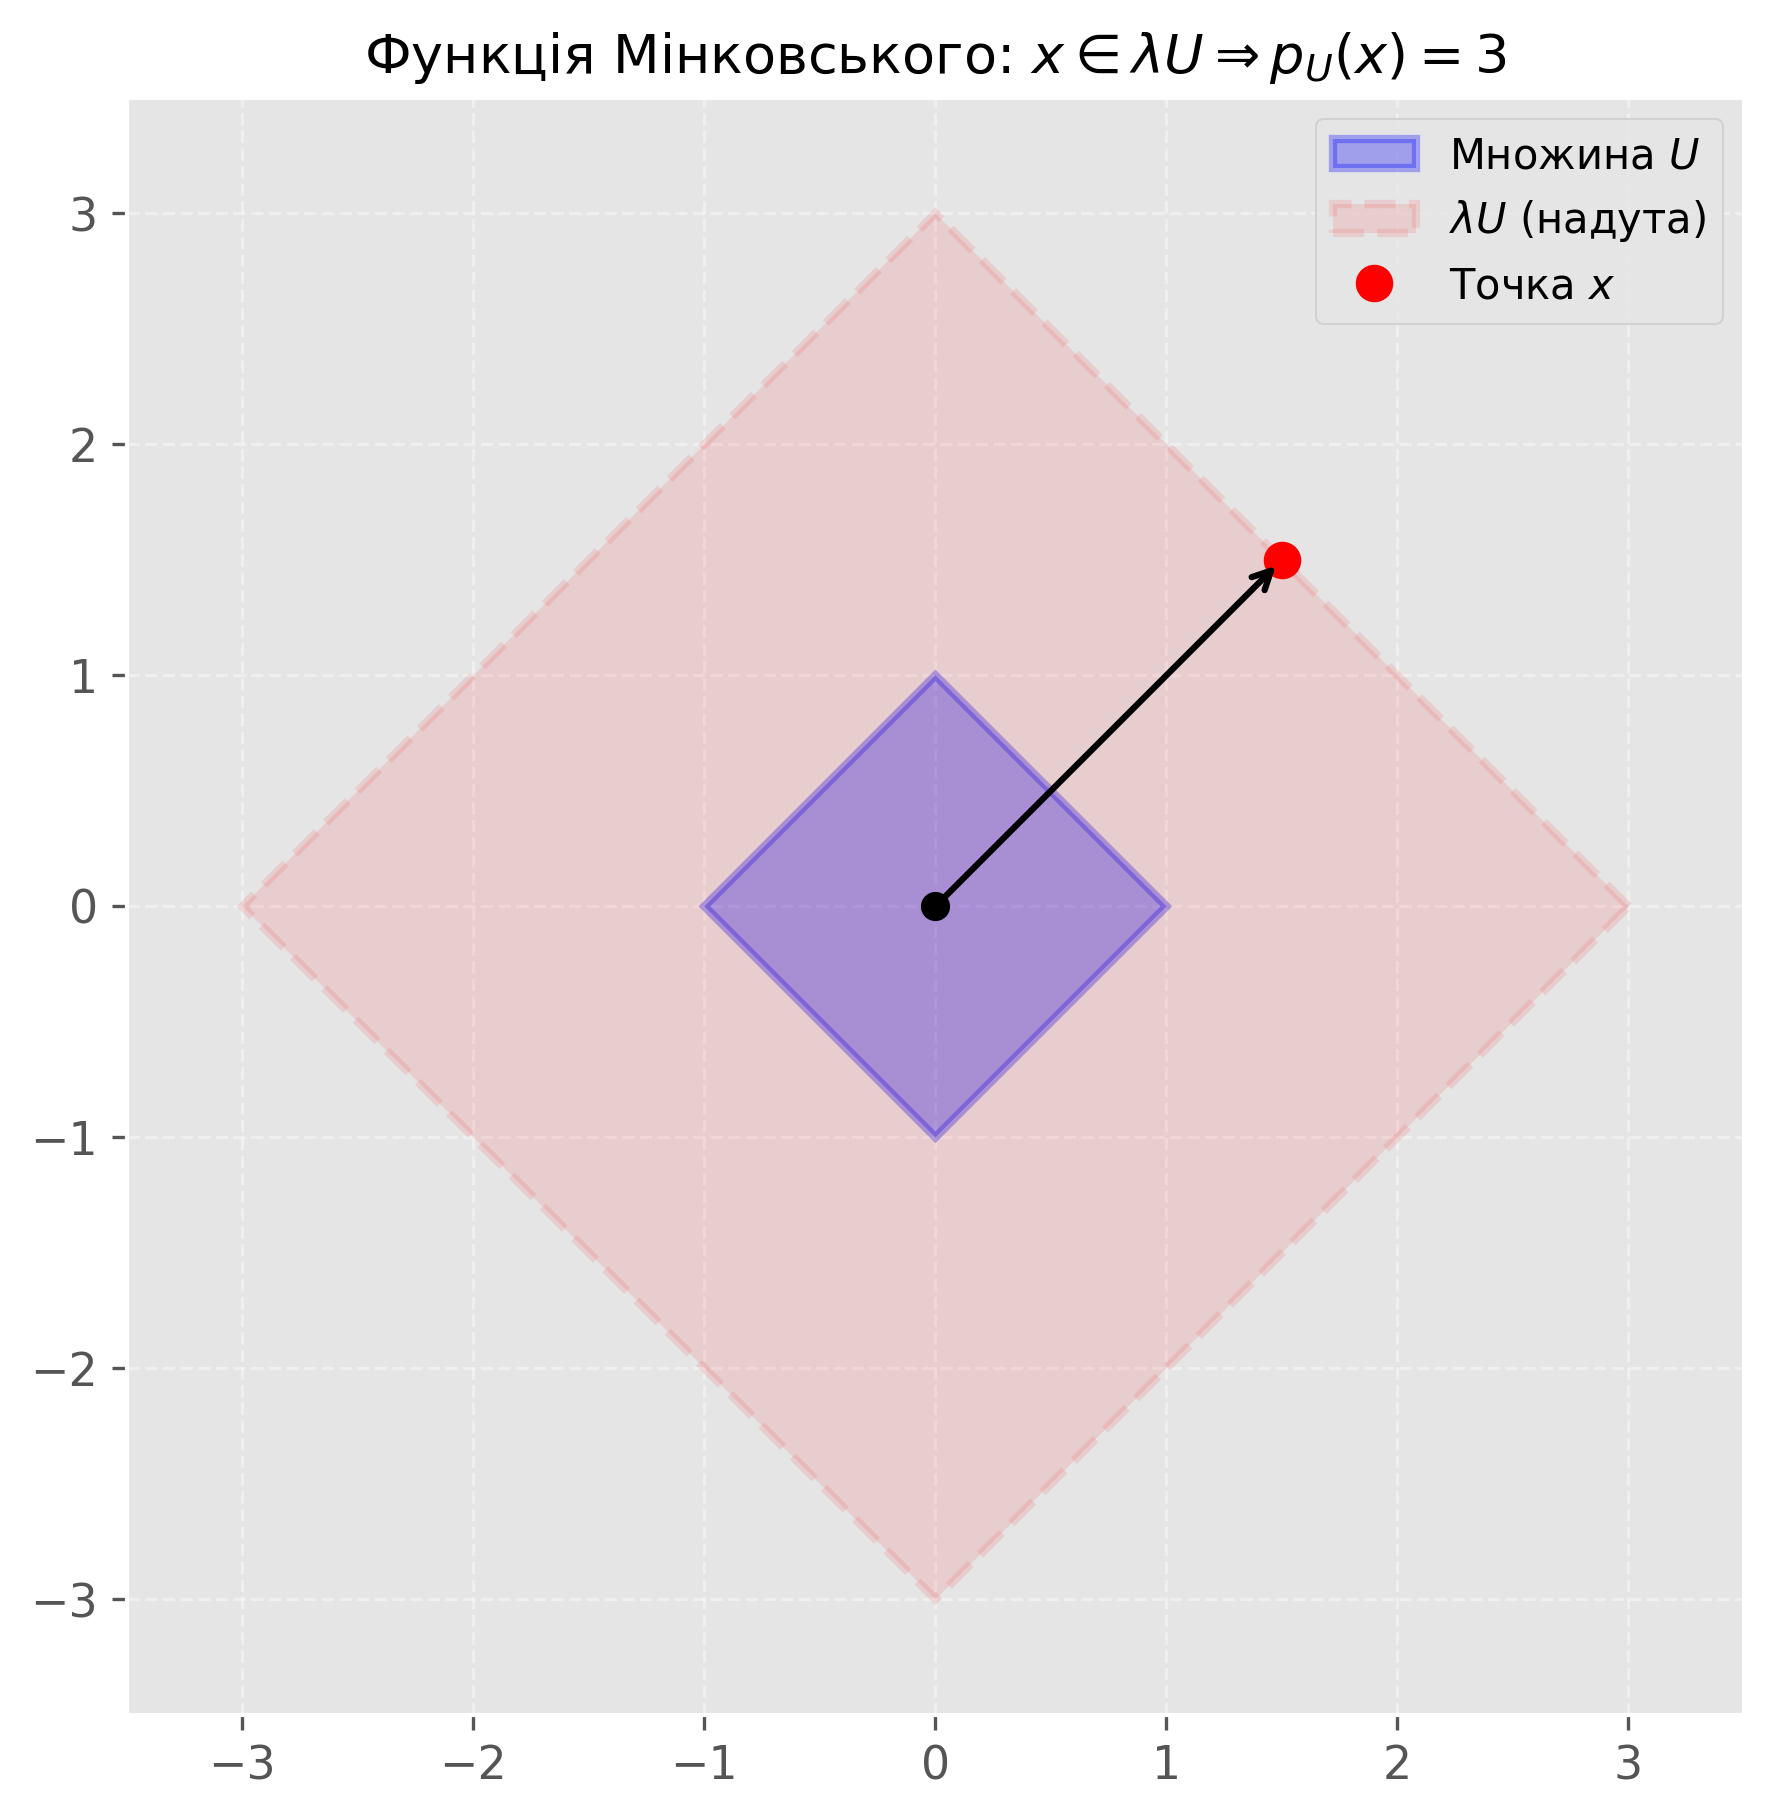
\includegraphics[width=0.7\textwidth]{minkowski_gauge.png}
\caption{Геометричний зміст функції Мінковського: коефіцієнт $\lambda$, на який треба розтягнути базову множину $U$, щоб вона досягла точки $x$.}
\label{fig:minkowski-gauge}
\end{figure}

Спряженою до функції Мінковського множини $A$ є індикаторна функція поляри $A^{0}$. Нехай $M$ --- опукла множина та $0 \in \operatorname{int} M$. Тоді функція Мінковського задовольняє такі властивості:\\
а) якщо $\lambda \geq 0$, то $\mu(\lambda x \mid M)=\lambda \mu(x \mid M)$;\\
б) якщо $x \in M$, то $\mu(x \mid M) \leq 1$, а якщо $x \notin M$, то $\mu(x \mid M) \geq 1$;\\
в) $\mu(x+y \mid M) \leq \mu(x \mid M)+\mu(y \mid M)$.

\section{Теорема Хана-Банаха.}
Нехай на просторі $X$ визначена функція $p(x)$ така, що

$$
p(x+y) \leq p(x)+p(y), \quad p(\lambda x)=\lambda p(x), \quad \lambda \geq 0 .
$$

Нехай, крім цього, задана лінійна функція $f(x)$ на підпросторі $X_{0} \subseteq X$ і $f(x) \leq p(x)$ для всіх $x \in X_{0}$. Тоді існує лінійна функція $F(x)$, що визначена на всьому просторі $X$ і така, що

$$
f(x)=F(x) \quad \text { для } x \in X_{0}
$$

і

$$
F(x) \leq p(x) \quad \text { для } x \in X \text {. }
$$

\part{Опуклі функції}

\section{Квазіопукла функція.}
Нехай $X$ --- опукла підмножина $\mathbb{R}^{n}$. Функцію $f: X \rightarrow \mathbb{R}$ називають квазіопуклою, якщо її множини Лебега

$$
X_{\beta}(f)=\{x \in X \mid f(x) \leq \beta\}
$$

є опуклими для всіх $\beta \in \mathbb{R}$.\\
Кожна опукла функція квазіопукла, однак зворотне твердження, загалом, хибне:

\begin{figure}[htbp]
\centering
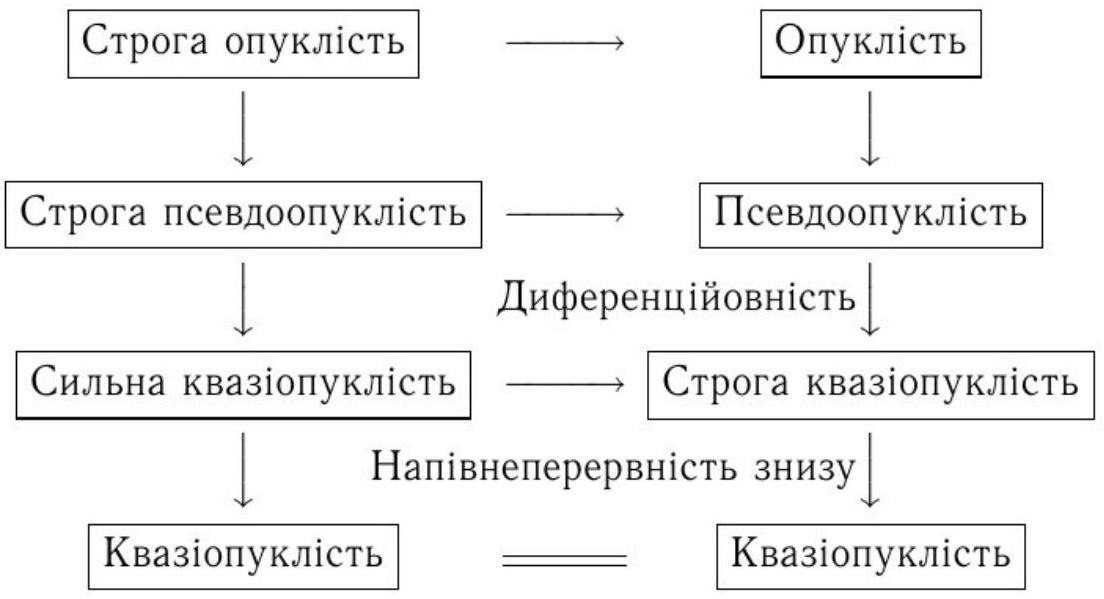
\includegraphics[width=0.85\textwidth]{6e2cc08c-e103-486e-965d-56342b3cf45f-3_599_1104_927_274}
\caption{Співвідношення між різними типами опуклості}
\label{fig:convexity-types}
\end{figure}

\section{Власна функція.}
Функцію називають власною, якщо вона не приймає значення $-\infty$ і не дорівнює тотожно $+\infty$. Для власної функції її ефективна множина непорожня.

\section{Ефективна множина функції.}
\textit{Ефективною множиною} функції $f$ називають множину точок, де $f$ приймає скінченні значення або $-\infty$:

$$
\operatorname{dom} f:=\left\{x \in \mathbb{R}^{n}: f(x)<\infty\right\}
$$

Ефективна множина опуклої функції (див. нижче) є опуклою

\section{Опукла функція.}
Функцію $f$ називають опуклою, якщо її надграфік $\operatorname{epi} f$ є опуклою множиною в $\mathbb{R}^{n} \times \mathbb{R}$. Для власної функції ця умова еквівалентна нерівності

$$
f\left(\lambda_{1} x_{1}+\lambda_{2} x_{2}\right) \leq \lambda_{1} f\left(x_{1}\right)+\lambda_{2} f\left(x_{2}\right), \quad \lambda_{1}, \lambda_{2} \geq 0, \quad \lambda_{1}+\lambda_{2}=1 .
$$

\section{Надграфік.}
\textit{Надграфік} (епіграф) функції $f: \mathbb{R}^{n} \rightarrow \mathbb{R} \cup\{-\infty\} \cup\{+\infty\}$ --- це множина

$$
\operatorname{epi} f:=\left\{(x, r) \in \mathbb{R}^{n} \times \mathbb{R}: f(x) \leq r\right\} \text {. }
$$

Значення функції відновлюють із надграфіка за формулою

$$
f(x)=\inf \{r \in \mathbb{R}:(x, r) \in \operatorname{epi} f\}
$$

\section{Додатньо однорідна функція.}
Функцію $p$ називають додатньо однорідною першого порядку, якщо

$$
p(\lambda x)=\lambda p(x), \quad \lambda>0 .
$$

\section{Нерівність Ієнсена.}
Для власної опуклої функції має місце

$$
f\left(\sum_{i=1}^{m} \lambda_{i} x_{i}\right) \leq \sum_{i=1}^{m} \lambda_{i} f\left(x_{i}\right), \quad \lambda_{i} \geq 0, \quad \sum_{i=1}^{m} \lambda_{i}=1 .
$$

\section{Опорна функція множини.}
Опорна функція є фундаментальним інструментом двоїстого опису опуклих множин через сімейство опорних гіперплощин.

\textbf{Означення.} \textit{Опорною функцією} непорожньої множини $X \subset \mathbb{R}^n$ називають функцію $W_X : \mathbb{R}^n \to \mathbb{R} \cup \{+\infty\}$, яка визначається як точна верхня грань скалярного добутку:
$$
W_X(p) = \sup_{x \in X} \langle p, x \rangle.
$$

\textbf{Основні властивості опорної функції:}
\begin{enumerate}
    \item $W_X(p)$ є опуклою та додатно-однорідною першого степеня ($W_X(\lambda p) = \lambda W_X(p)$ для всіх $\lambda > 0$), тобто сублінійною функцією.
    \item Опорна функція $X$ збігається з опорною функцією $\operatorname{conv} X$ та $\overline{X}$: $W_X(p) = W_{\operatorname{conv} X}(p) = W_{\overline{X}}(p)$.
    \item Множина $X$ є обмеженою тоді і тільки тоді, коли її опорна функція набуває лише скінченних значень для всіх $p \in \mathbb{R}^n$.
\end{enumerate}

\section{Поляра множини.}
Поляра множини $A$ визначається за допомогою опорної функції:

$$
A^{0}=\left\{x^{*} \in X^{*}: s\left(x^{*} \mid A\right) \leq 1\right\} .
$$

Для конуса $K$ маємо

$$
K^{0}=\left\{x^{*} \in X^{*}:\left\langle x^{*}, x\right\rangle \leq 0, \forall x \in K\right\} .
$$

\section{Критерії опуклості диференційовних функцій.}
Нехай $f(x)$ диференційовна. Еквівалентні такі умови опуклості:\\
(i) функція $f$ опукла;\\
(ii) для всіх $x, \hat{x} \in \mathbb{R}^{n}$

$$
f(x)-f(\hat{x}) \geq\left\langle f^{\prime}(\hat{x}), x-\hat{x}\right\rangle ;
$$

(iii) для всіх $x, \hat{x} \in \mathbb{R}^{n}$

$$
\left\langle f^{\prime}(x)-f^{\prime}(\hat{x}), x-\hat{x}\right\rangle \geq 0 ;
$$

(iiii) функція $\left\langle p, f^{\prime}(x+\alpha p)\right\rangle$ неспадна як функція від $\alpha \in \mathbb{R}$ для всіх $x \in \mathbb{R}^{n}$ та $p \in \mathbb{R}^{n}$;\\
(iiiii) за умови, що функція $f(x)$ двічі неперервно диференційовна:

$$
\left\langle f^{\prime \prime}(x) h, h\right\rangle \geq 0 \quad \text { для всіх } x, h \in \mathbb{R}^{n} .
$$

\section{Неперервність опуклих функцій і умова Ліпшиця.}
Якщо власна опукла функція обмежена зверху в деякому околі точки $\widehat{x}$, то вона неперервна в цій точці. Якщо опукла функція неперервна в точці $\widehat{x}$, то вона задовольняє умову Ліпшиця в деякому околі цієї точки:

$$
|f(x)-f(\widehat{x})| \leq L\|x-\widehat{x}\|
$$

\section{Замкнута та напівнеперервна знизу функція.}
Функція

$$
f: \mathbb{R}^{n} \rightarrow \mathbb{R} \cup\{+\infty\}
$$

називають замкнутою, якщо її надграфік $\operatorname{epi} f$ є замкнутою множиною в $\mathbb{R}^{n} \times \mathbb{R}$ :

$$
\operatorname{epi} f=\left\{(x, r) \in \mathbb{R}^{n} \times \mathbb{R} \mid f(x) \leq r\right\} \text {. }
$$

Для функції $f$ наступні властивості еквівалентні:\\
(i) функція $f$ напівнеперервна знизу на $\mathbb{R}^{n}$;\\
(ii) функція $f$ замкнута;\\
(iii) $S_{r}(f)=\left\{x \in \mathbb{R}^{n}: f(x) \leq r\right\}$ замкнуті в $\mathbb{R}^{n}$ для всіх $r \in \mathbb{R}$.

\textit{Замиканням} (напівнеперервною знизу оболонкою) функції

$$
f: \mathbb{R}^{n} \rightarrow \mathbb{R} \cup\{ \pm \infty\}
$$

визначається співвідношенням

$$
\operatorname{cl} f(x)=\liminf _{y \rightarrow x} f(y), \quad \forall x \in \mathbb{R}^{n}
$$

або, еквівалентно,

$$
\operatorname{epi}(\operatorname{cl} f)=\operatorname{cl}(\operatorname{epi} f)
$$

\section{Конволюція функцій.}
\textit{Інфімальну конволюцію} власних опуклих функцій $f_{1}, \ldots, f_{m}$ визначають формулою

$$
\left(\oplus_{i=1}^{m} f_{i}\right)(x)=\inf \left\{\sum_{i=1}^{m} f_{i}\left(x_{i}\right): \sum_{i=1}^{m} x_{i}=x\right\}
$$

\section{Верхня грань функцій.}
Для сім'ї опуклих функцій $f_{i}, і \in I$, верхня грань задається як

$$
f(x)=\left(\vee_{i \in I} f_{i}\right)(x)=\sup _{i \in I} f_{i}(x)
$$

Верхня грань сім'ї опуклих функцій також є опуклою функцією.

\section{Нижня грань функцій та опукла оболонка нижньої грані.}
Нижню грань функцій визначають через опуклу оболонку:

$$
f(x)=\left(\operatorname{conv}\left(\wedge_{i \in I}\right) f_{i}\right)(x)=\inf \left\{\alpha \in \mathbb{R}:(x, \alpha) \in \operatorname{conv}\left(\cup_{i \in I} \text { epi } f_{i}\right)\right\}
$$

\section{Спряжена функція. Перетворення Юнга-Фенхеля.}
Спряжена функція до $f$ визначається формулою

$$
f^{*}\left(x^{*}\right)=\sup _{x}\left\{\left\langle x^{*}, x\right\rangle-f(x)\right\} .
$$

\begin{figure}[htbp]
\centering
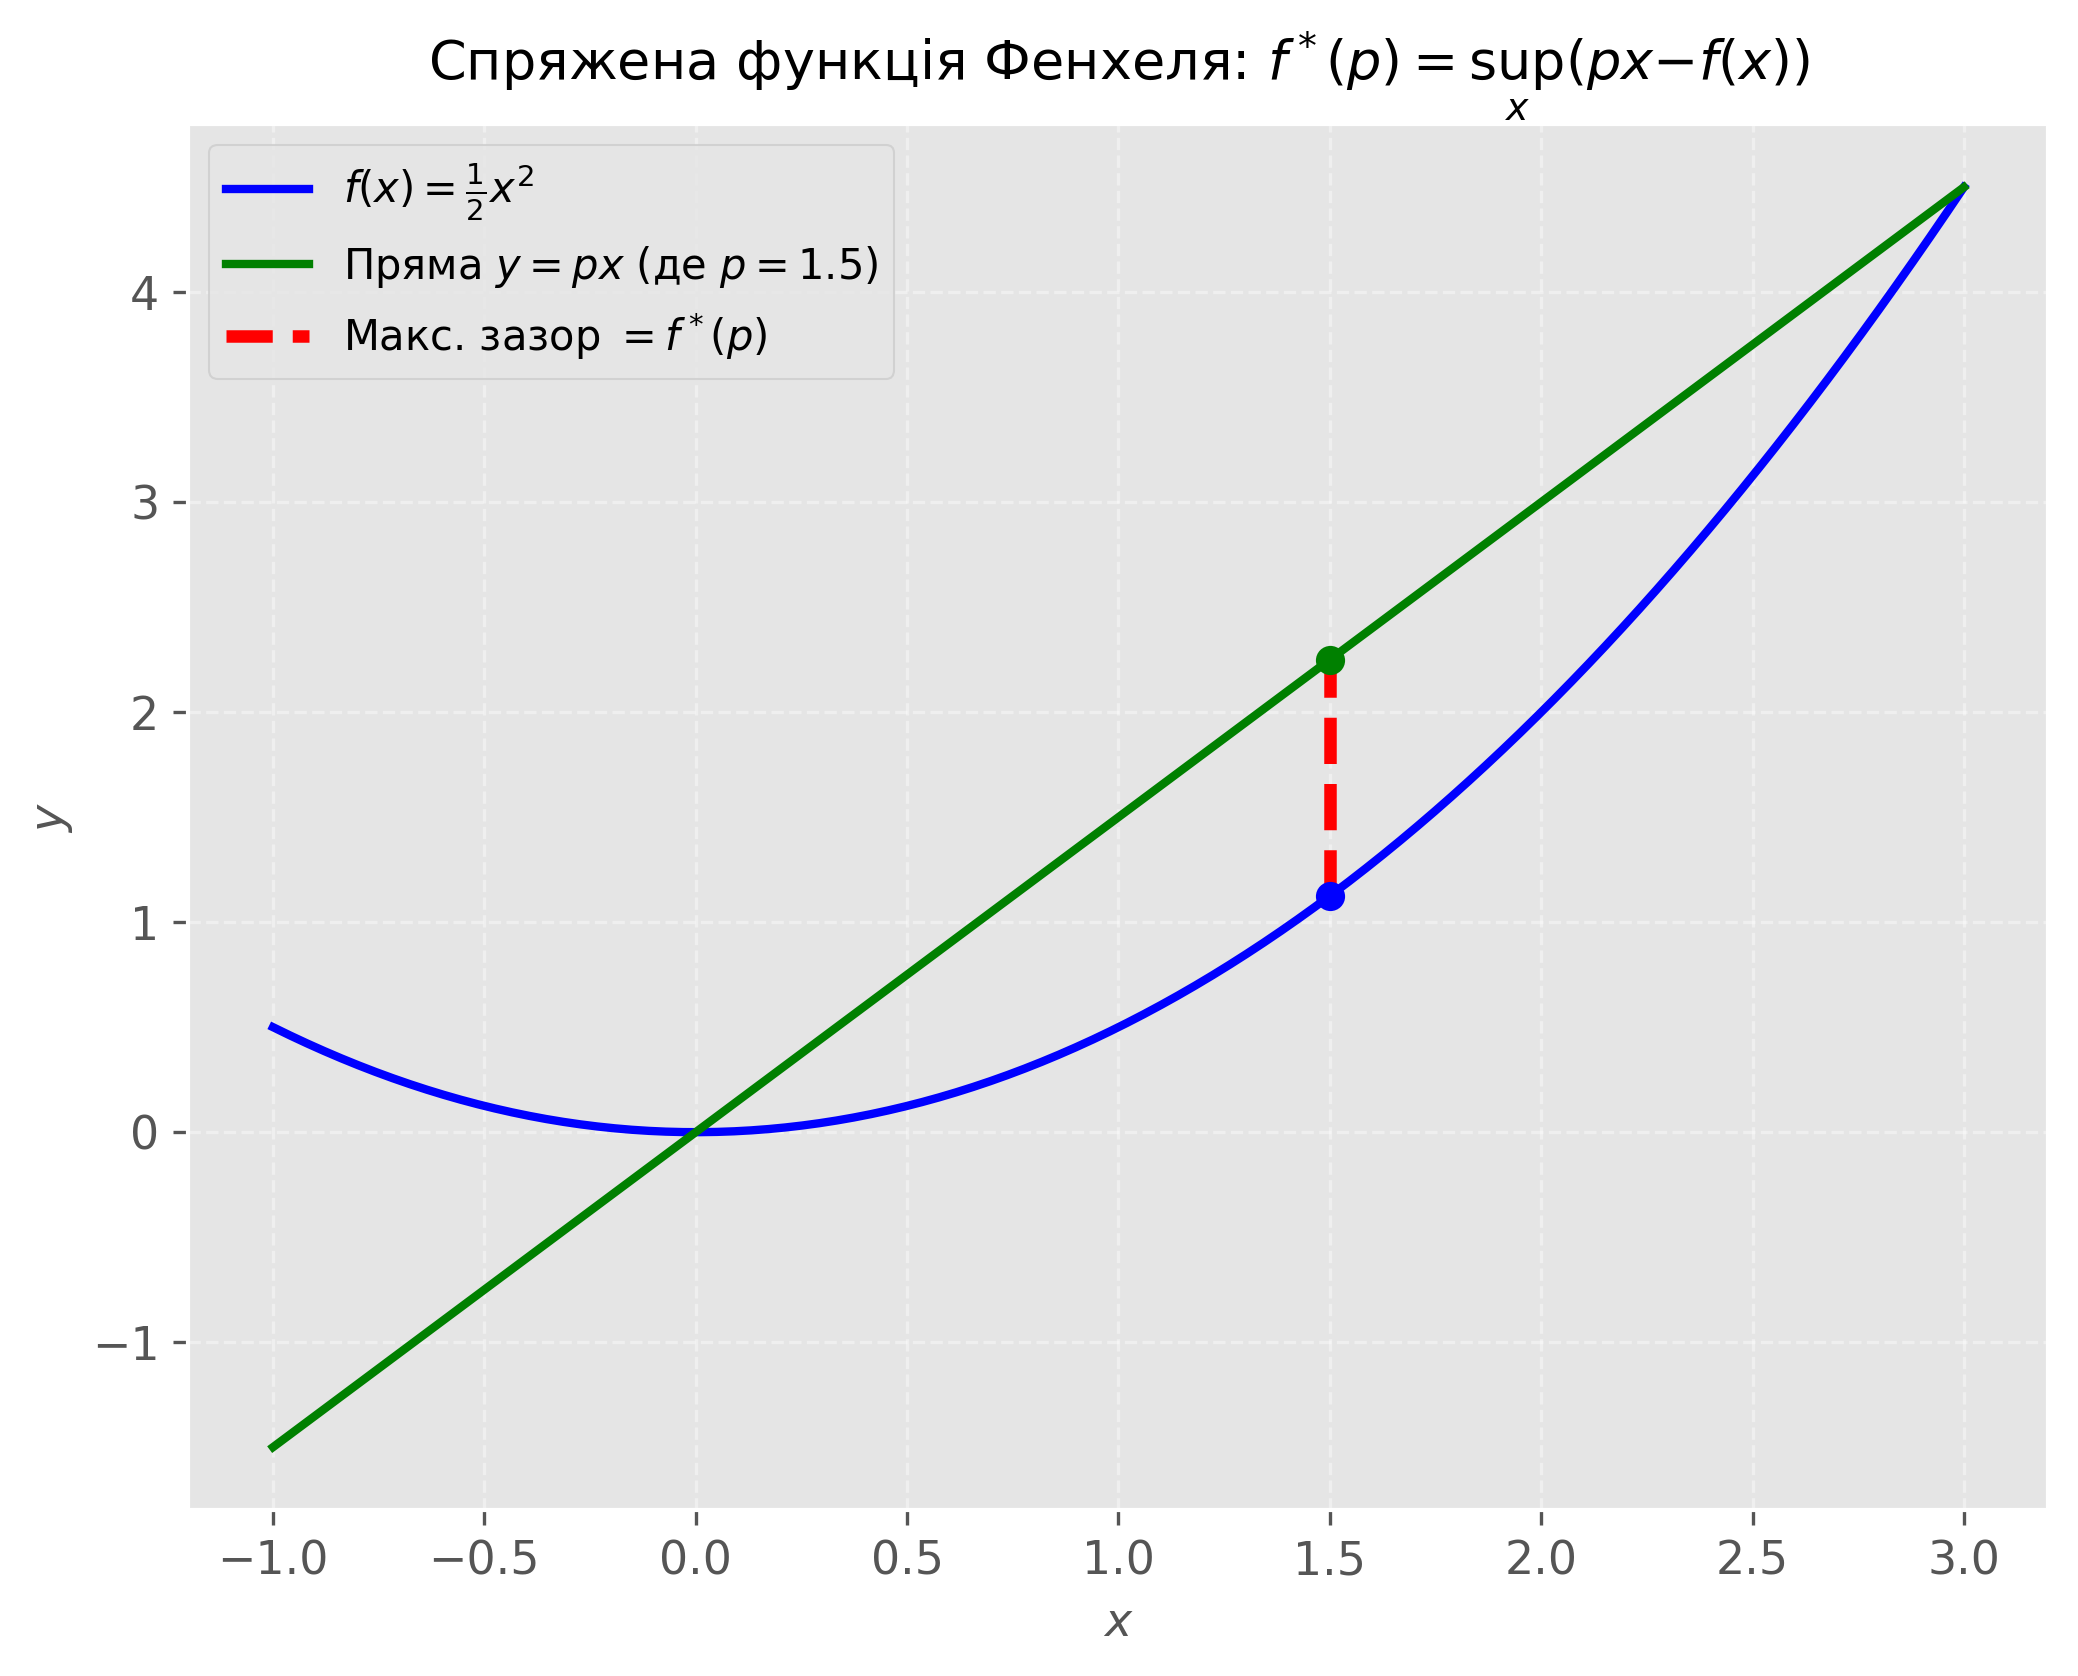
\includegraphics[width=0.85\textwidth]{fenchel_conjugate.png}
\caption{Перетворення Лежандра-Фенхеля: значення $f^*(p)$ дорівнює максимальній вертикальній відстані (зазору) між прямою $y = px$ та графіком функції $f(x)$.}
\label{fig:fenchel-conjugate}
\end{figure}

Це перетворення також називають перетворенням Юнга-Фенхеля функції $f$.\\
Якщо $f(x)$ --- опукла гладка функція на $\mathbb{R}^{n}$, що росте на нескінченності швидше лінійної функції, перетворення Юнга-Фенхеля збігається з перетворенням Лежандра:

$$
f^{*}\left(x^{*}\right)=\left\langle x^{*}, x_{0}\right\rangle-f\left(x_{0}\right),
$$

\section{Нерівність Юнга-Фенхеля.}
Для всіх $x \in X$ і $x^{*} \in X^{*}$ справджується нерівність

$$
f(x)+f^{*}\left(x^{*}\right) \geq\left\langle x^{*}, x\right\rangle
$$

\section{Теорема Фенхеля-Моро.}
Нехай $f$ --- функція на $X$, що скрізь приймає значення більші за $-\infty$. Тоді $f=f^{* *}$ тоді і тільки тоді, коли $f$ опукла і замкнута.

\section{Теорема Ферма для опуклої функції.}
Для негладких опуклих функцій класичне диференціальне числення замінюється апаратом субдиференціалів, що дозволяє сформулювати критерій оптимуму без вимоги гладкості.

\textbf{Теорема (Узагальнена теорема Ферма).} Нехай $f: \mathbb{R}^n \to \mathbb{R} \cup \{+\infty\}$ --- власна опукла функція. Точка $x^* \in \mathbb{R}^n$ є точкою глобального мінімуму цієї функції на $\mathbb{R}^n$ тоді і тільки тоді, коли нульовий вектор належить її субдиференціалу в цій точці:
$$
0 \in \partial f(x^*).
$$

\textbf{Доведення.} За означенням субдиференціала, включення $0 \in \partial f(x^*)$ означає, що для всіх $x \in \mathbb{R}^n$ виконується нерівність:
$$
f(x) - f(x^*) \geq \langle 0, x - x^* \rangle \implies f(x) \geq f(x^*).
$$
Ця нерівність тотожна означенню точки глобального мінімуму, що й треба було довести.

\section{Похідна за напрямком.}
Похідна функції $f$ у точці $x$ за напрямком $p$ визначається як

$$
f^{\prime}(x, p)=\lim _{\lambda \Downarrow 0} \frac{f(x+\lambda p)-f(x)}{\lambda},
$$

якщо ця границя існує.

\section{Субградієнт і субдиференціал.}
Вектор $x^{*} \in X^{*}$ називають субградієнтом функції $f$ у точці $x_{0}$, якщо

$$
f(x)-f\left(x_{0}\right) \geq\left\langle x^{*}, x-x_{0}\right\rangle \quad \forall x \in X .
$$

Множину всіх субградієнтів називають субдиференціалом функції $f$ у точці $x_{0}$ і позначається $\partial f\left(x_{0}\right)$.

\begin{figure}[htbp]
\centering
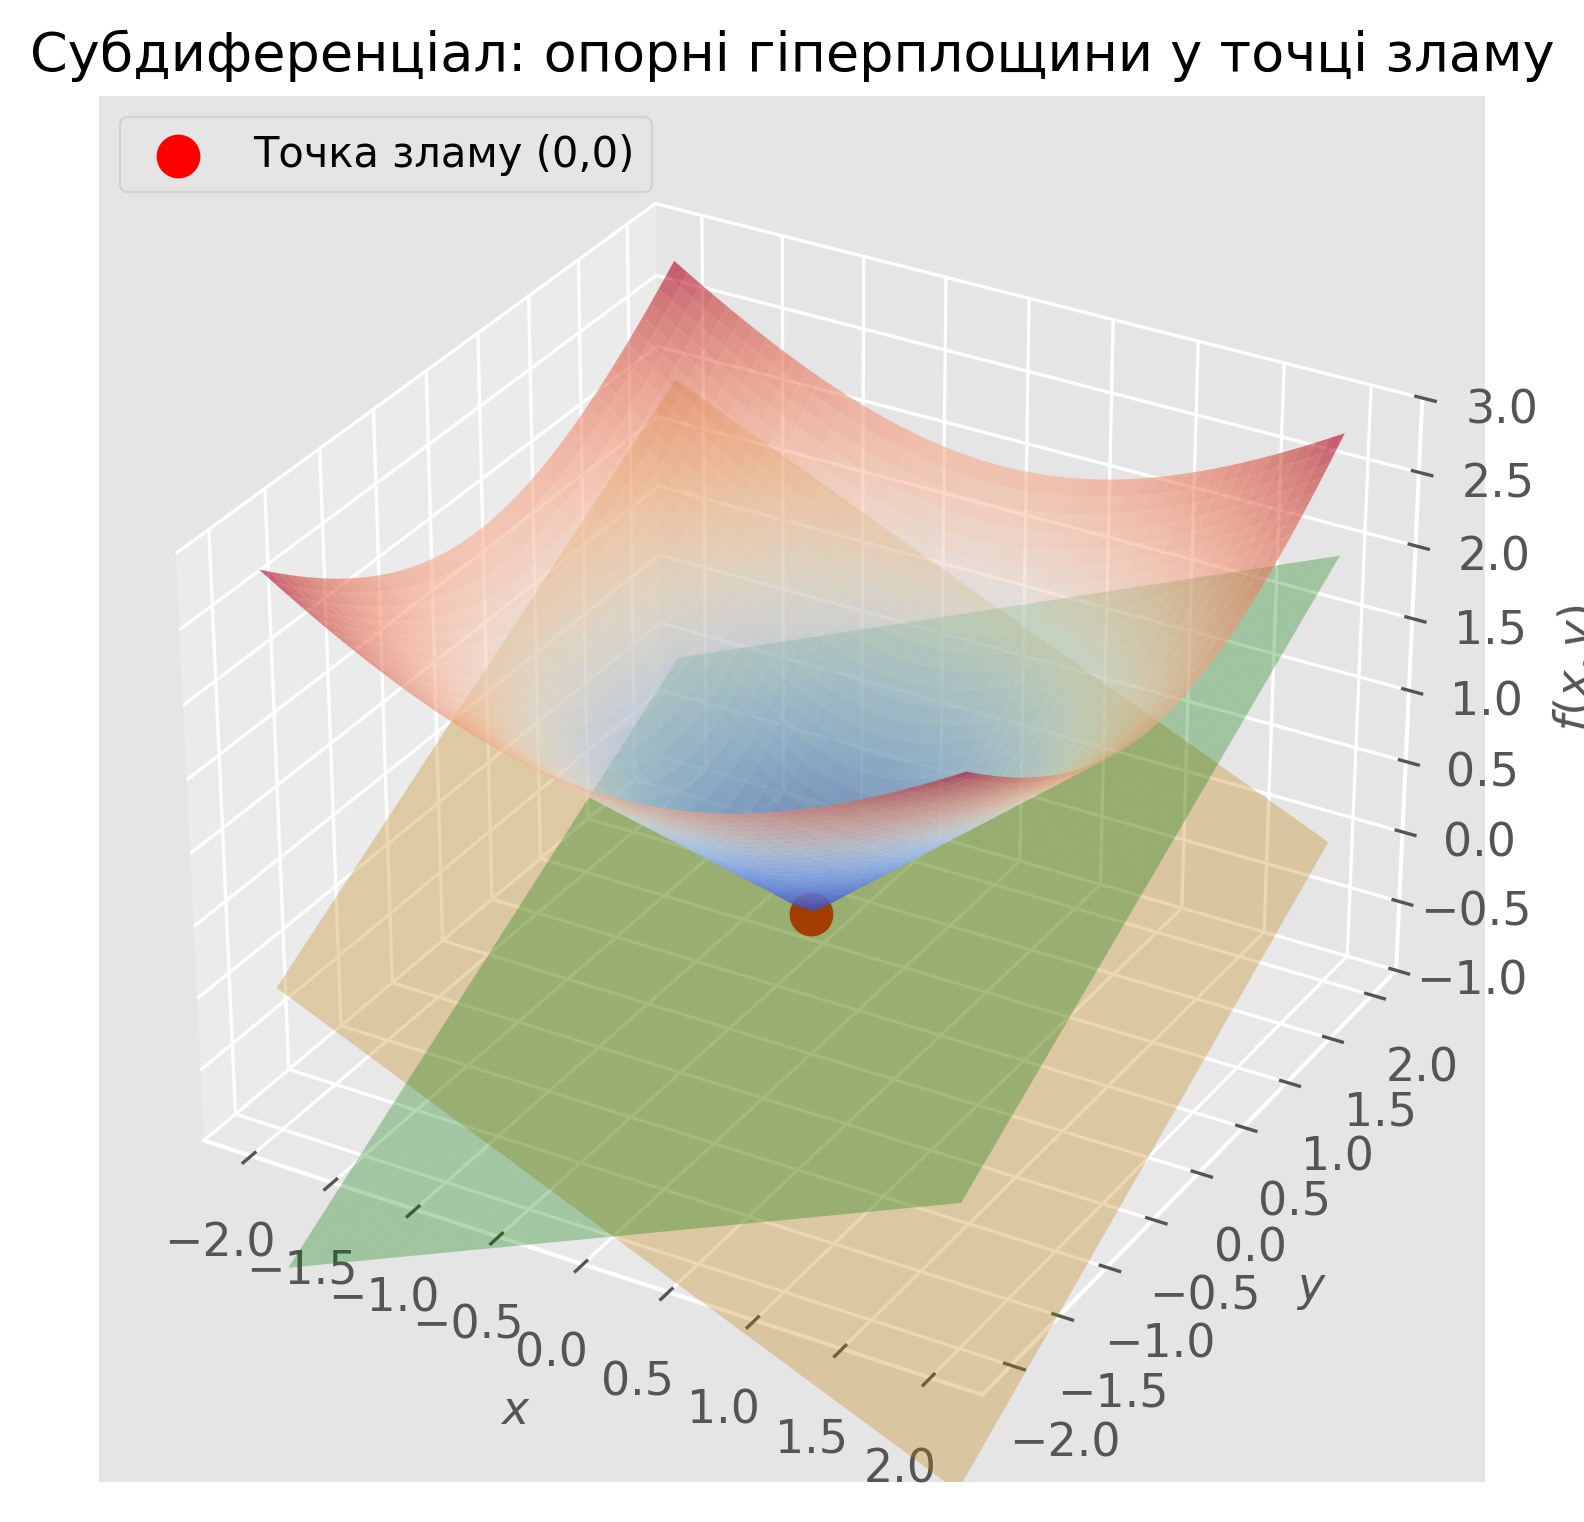
\includegraphics[width=0.9\textwidth]{subgradient_3d.png}
\caption{Геометричний зміст субдиференціала: пучок опорних площин у негладкій точці конуса.}
\label{fig:subgradient-3d}
\end{figure}

\section{Субдиференціал і похідна за напрямком опуклої функції.}
Для опуклої функції $f$, неперервної в $x_{0}$, субдиференціал $\partial f\left(x_{0}\right)$ --- непорожня, замкнутою, опуклою і обмеженою множиною, причому

$$
f^{\prime}\left(x_{0}, p\right)=\max _{x^{*} \in \partial f\left(x_{0}\right)}\left\langle p, x^{*}\right\rangle .
$$

Якщо $f$ диференційовна в точці $x_{0}$, то

$$
\partial f\left(x_{0}\right)=\left\{f^{\prime}\left(x_{0}\right)\right\} .
$$

\section{Теорема Моро-Рокафеллара.}
Нехай $f_{1}, \ldots, f_{n}$ --- власні опуклі функції на $X$. Тоді для кожної точки $x \in X$

$$
\partial f_{1}(x)+\cdots+\partial f_{n}(x) \subset \partial\left(f_{1}+\cdots+f_{n}\right)(x)
$$

Якщо в деякій точці $x_{1} \in\left(\operatorname{dom} f_{1}\right) \cap \cdots \cap\left(\operatorname{dom} f_{n}\right)$ функції $f_{1}(x), \ldots, f_{n}(x)$, за виключенням може однієї, неперервні, то

$$
\partial f_{1}(x)+\cdots+\partial f_{n}(x)=\partial\left(f_{1}+\cdots+f_{n}\right)(x)
$$

для всіх $x \in X$.

\section{Субдиференціал індикаторної функції.}
Для індикаторної функції $\delta(x \mid M)$ опуклої множини $M$ та точки $x_{0} \in M$ виконується

$$
\partial \delta\left(x_{0} \mid M\right)=-\left(\operatorname{cone}\left(M-x_{0}\right)\right)^{*} .
$$

\section{Субдиференціал максимуму функцій.}
Нехай $f(x)=\max _{i=1, \ldots, m} f_{i}(x)$, де кожна $f_{i}$ --- опукла та неперервна в $x_{0}$. Тоді

$$
\partial f\left(x_{0}\right)=\operatorname{conv}\left(\bigcup_{i \in I\left(x_{0}\right)} \partial f_{i}\left(x_{0}\right)\right),
$$

де

$$
I\left(x_{0}\right)=\left\{i: f_{i}\left(x_{0}\right)=f\left(x_{0}\right)\right\} .
$$

\begin{figure}[htbp]
\centering
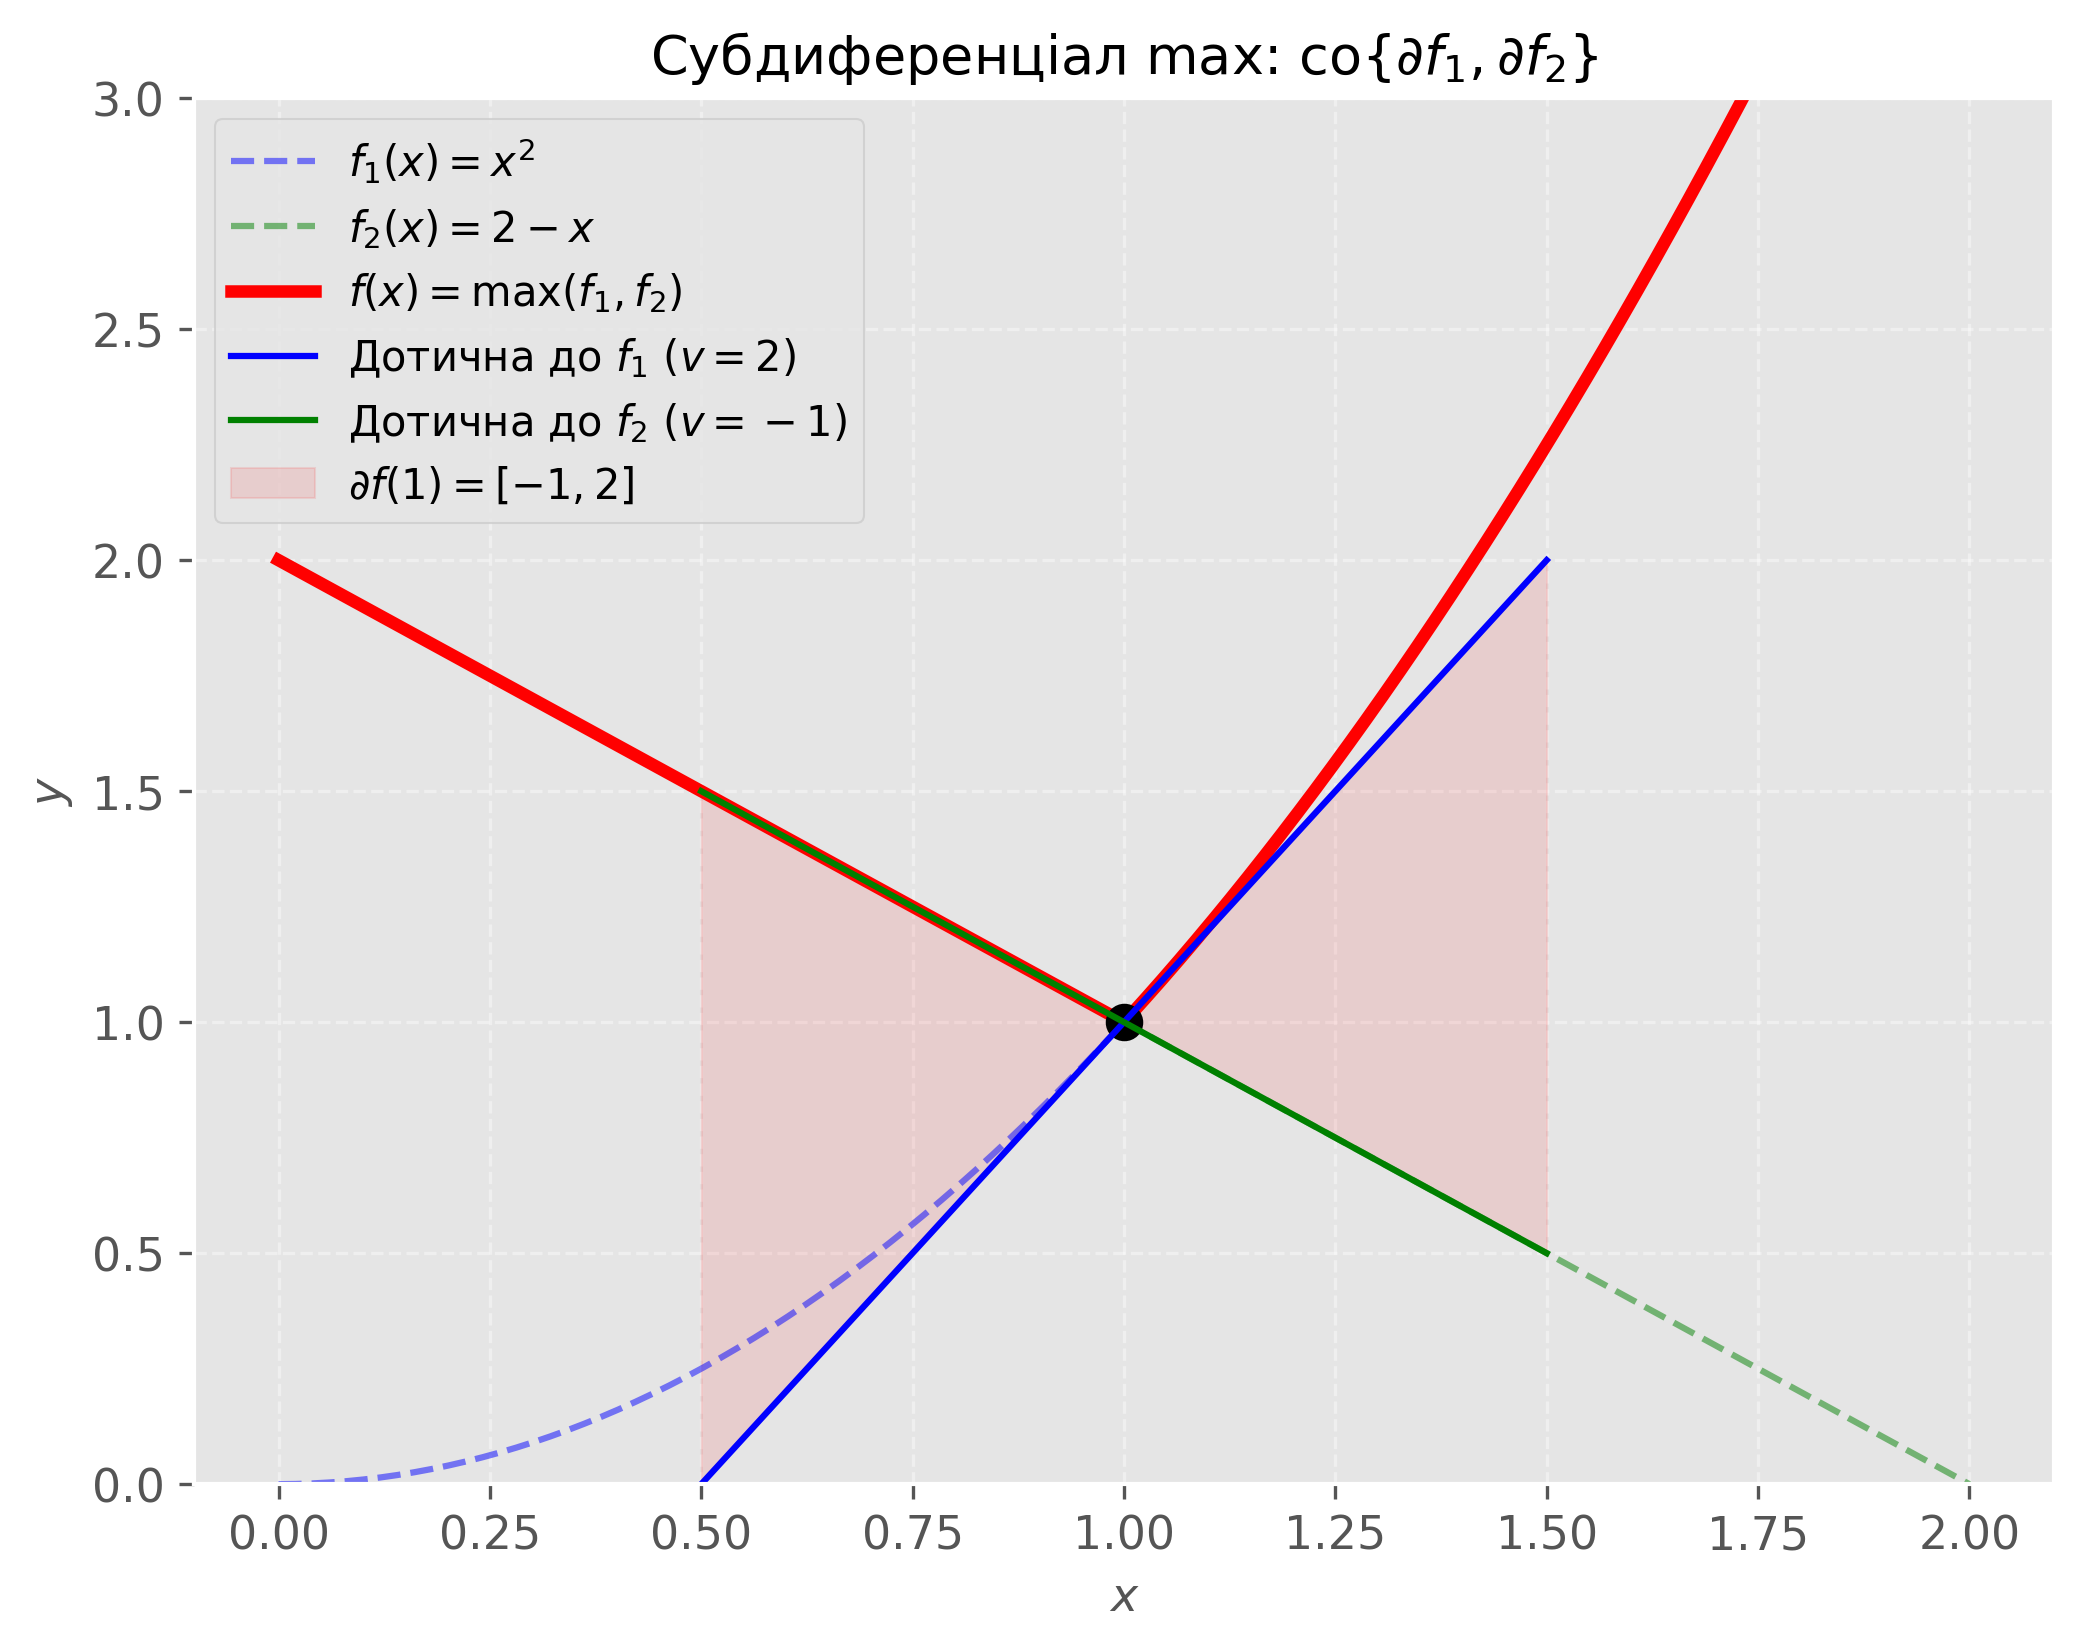
\includegraphics[width=0.85\textwidth]{max_subdifferential.png}
\caption{Субдиференціал максимуму двох функцій є опуклою оболонкою їхніх дотичних у точці перетину (зламу), утворюючи суцільне «віяло» опорних прямих.}
\label{fig:max-subdifferential}
\end{figure}

\section{Субдиференціал композиції функцій.}
Нехай $\Lambda: X \rightarrow Y$ --- неперервний лінійний оператор, $f$ --- опукла функція на $Y$. Тоді для кожної точки $x \in X$ справджується

$$
\Lambda^{*} \partial f(\Lambda x) \subset \partial(f \Lambda)(x)
$$

Якщо функція $f$ неперервна в деякій точці $y_{0} \in \operatorname{Im} \Lambda$, то для кожної точки $x \in X$ справджується рівність

$$
\Lambda^{*} \partial f(\Lambda x)=\partial(f \Lambda)(x)
$$

Нехай $g_{1}, \ldots, g_{m}$ --- опуклі функції на $X$, $g=\left(g_{1}, \ldots, g_{m}\right)$ --- відповідна вектор-функція, $\varphi$ --- монотонно неспадна опукла функція на відкритій опуклій множині $U \subset \mathbb{R}^{m}, g(X) \subset U$. Якщо функція $g(x)$ неперервна в точці $x_{0}$, а функція $\varphi$ неперервна в точці $g\left(x_{0}\right)$, то субдиференціал функції $f\left(x_{0}\right)=\varphi\left(g\left(x_{0}\right)\right)$ має вигляд

$$
\partial f\left(x_{0}\right)=\bigcup_{p \in \partial \varphi(u)}\left(\sum_{i=1}^{m} p_{i} \partial g_{i}\left(x_{0}\right)\right),
$$

де $u=g\left(x_{0}\right)$.\\
Якщо $\varphi$ диференційовна в $u=g\left(x_{0}\right)$, отримуємо

$$
\partial f\left(x_{0}\right)=\sum_{i=1}^{m} \frac{\partial \varphi}{\partial u_{i}}\left(g\left(x_{0}\right)\right) \partial g_{i}\left(x_{0}\right) .
$$

Якщо також $g_{1}, \ldots, g_{m}$ диференційовні в $x_{0}$, випливає класична формула градієнта суперпозиції:

$$
f^{\prime}\left(x_{0}\right)=\sum_{i=1}^{m} \frac{\partial \varphi}{\partial u_{i}}\left(g\left(x_{0}\right)\right) g_{i}^{\prime}\left(x_{0}\right) .
$$

\textbf{Функція відстані до множини.}\\
Нехай $M$ --- опукла множина, $C$ --- опукла обмежена множина, $0 \in \operatorname{int} C$. Тоді для всіх $x \in X$ визначена функція

$$
d_{C}(x \mid M)=\inf _{\rho}\{\rho \geq 0: x \in M+\rho C\}
$$

Якщо $C=B$, де $B$ --- одинична куля з центром у нулі, то $d_{B}(x \mid M)$ --- відстань від точки $x$ до множини $M$. Якщо $M=\{0\}$, то

$$
d_{C}(x \mid\{0\})=\inf _{\rho}\{(\rho>0: x \in \rho C)\}=\inf _{\rho}\left\{\left(\rho>0: \frac{x}{\rho} \in C\right)\right\}=\mu(x \mid C),
$$

де $\mu(x \mid C)$ --- функція Мінковського.

% ==========================================
% ДОДАТКОВІ СЕКЦІЇ ДО РОЗДІЛУ 2 (ОПУКЛІ ФУНКЦІЇ)
% ==========================================

\part{Верхня опукла апроксимація}

\section{Конус дотичних напрямків.}
Конус дотичних напрямків описує ті напрямки, у яких можна локально рухатися від точки множини з малою поправкою.

Вектор $g \in X$ називають \textit{дотичним} до $M$ у $x \in M$, якщо існує функція $\varphi(\lambda) \in X$, що

$$
x+\lambda g+\varphi(\lambda) \in M
$$

при достатньо малих $\lambda \geq 0$ і $\lambda^{-1} \varphi(\lambda) \rightarrow 0$ коли $\lambda \downarrow 0$.\\
Множина дотичних напрямків, як правило, утворює конус: разом із $g$ дотичним є й $\alpha g$ при $\alpha \geq 0$.\\
Опуклий конус $K(x, M)$ називають \textit{конусом дотичних напрямків} до $M$ у $x$, якщо з $g \in K(x, M)$ випливає, що $g$ --- дотичний вектор до $M$ у $x \in M$.

Якщо $M$ --- опукла, то

$$
K(x, M)=\operatorname{cone}(M-x)=\{g: g=\lambda(y-x), y \in M, \lambda>0\}
$$

є конусом дотичних напрямків до $M$. Для цього достатньо покласти $\varphi(\lambda) \equiv 0$ в означенні.

\section{Шатра.}
Конус дотичних напрямків містить напрямки, для кожного з яких в означенні існує своя функція $\varphi(\lambda)$. Цього виявляється недостатньо для того, щоб робити висновки про властивості множини $M$.

Конус дотичних напрямків $K\left(x_{0}, M\right)$ в точці $x_{0} \in M$ називають локальним шатром, якщо для кожного напрямку $g \in \operatorname{ri} K\left(x_{0}, M\right)$ існує опуклий конус $Q$ і визначене в околі початку координат неперервне відображення $\psi(g)$ такі, що:

$$
\begin{aligned}
& \text { а) } \quad g \in \operatorname{ri} Q, \quad \operatorname{Lin} Q=\operatorname{Lin} K\left(x_{0}, M\right), \quad Q \subseteq K\left(x_{0}, M\right) ; \\
& \text { б) } \psi(g)=g+r(g), \quad\|g\|^{-1} r(g) \rightarrow 0 \quad \text { при } g \rightarrow 0 ; \\
& \text { в) } \quad x_{0}+\psi(g) \in M \quad \text { для } g \in Q \cap(\varepsilon B) \quad \text { при деякому } \varepsilon>0 .
\end{aligned}
$$

$B$ --- одинична куля в $X=\mathbb{R}^{n}$.

\section{Похідна Пшеничного.}
Для $x \in \operatorname{dom} f=\{x:|f(x)|<+\infty\} ., g \neq 0$

$$
F(x, g)=\sup _{r(\cdot)} \limsup _{\lambda \downarrow 0} \frac{f(x+\lambda g+r(\lambda))-f(x)}{\lambda}, \quad \frac{r(\lambda)}{\lambda} \rightarrow 0 .
$$

де зовнішня верхня грань береться по всім функціям $r(\lambda) \in X$ таким, що $\lambda^{-1} r(\lambda) \rightarrow 0$ при $\lambda \downarrow 0$, називають \textit{похідною за напрямком Пшеничного}. Величина $F(x, g)$ завжди існує (скінченна або нескінченна).\\
Легко також перевірити, що функція $F(x, g)$ додатньо однорідна за $g$, тобто для $\lambda>0$

$$
F(x, \lambda g)=\lambda F(x, g) .
$$

Якщо виконується умова Ліпшиця в околі точки $x$, справедлива формула

$$
F(x, g)=\underset{\lambda \downarrow 0}{\lim \sup } \frac{f(x+\lambda g)-f(x)}{\lambda} .
$$

\section{Верхня опукла апроксимація. (в. о. а)}
Функцію $h(x, g)$ називають верхньою опуклою апроксимацією функції $f$ у точці $x$, якщо вона мажорує похідну Пшеничного за ненульовими напрямками і як функція $h(x, g)$ є опуклою, замкнутою та додатньо однорідною:

$$
h(x, g) \geq F(x, g), \quad g \neq 0
$$

Якщо $h_{1}(x, g)$ і $h_{2}(x, g)$ --- в.о.а. $f$ у $x$, то також в.о.а. є

$$
h(x, g)=\lambda_{1} h_{1}(x, g)+\lambda_{2} h_{2}(x, g), \quad \lambda_{1}+\lambda_{2}=1, \quad \lambda_{1}, \lambda_{2} \geq 0
$$

і функція

$$
h(x, g)=\max \left\{h_{1}(x, g), h_{2}(x, g)\right\}
$$

також є в.о.а. для $f(x)$ в точці $x$.

\section{Субдиференціал, породжений верхньою опуклою апроксимацією.}
Якщо $h(x, g)$ є верхньою опуклою апроксимацією, то субдиференціал визначається як

$$
\partial f(x)=\partial h(x, 0)=\left\{x^{*}: h(x, g) \geq\left\langle x^{*}, g\right\rangle, \forall g\right\} .
$$

При цьому

$$
h(x, g)=\sup _{x^{*} \in \partial f(x)}\left\langle x^{*}, g\right\rangle
$$

\section{Головна верхня апроксимація і головний субдиференціал.}
В.о.a. $h(x, g)$ функції $f(x)$ в точці $x$ називають головною, якщо не існує іншої в.о.а. $h_{1}(x, g)$, такої, що

$$
h(x, g) \geq h_{1}(x, g) \quad \forall x .
$$

Відповідний субдиференціал називають головним.\\
Якщо $F(x, g)$ після довизначення $F(x, 0)=0$ --- опукла замкнута функція, головний субдиференціал єдиний. Для опуклої неперервної $f$ звичайний субдиференціал збігається з головним.\\
Якщо $h(x, g)=\left\langle x^{*}, g\right\rangle$ є в.о.а. функції $f$ в точці $x$, то $h(x, g)$ --- головна в.о.а., а $x^{*}$ --- головний субдиференціал.

\part{Похідні за напрямком}

\section{Похідна Діні.}
Нехай функція $f: \mathbb{R}^{n} \rightarrow \mathbb{R}^{1}$ визначена на деякій відкритій множині $S \subset \mathbb{R}^{n}$ і приймає лише скінченні значення.\\
Величина

$$
f_{D}^{\uparrow}(x, g)=\varlimsup_{\alpha \downarrow 0} \frac{1}{\alpha}(f(x+\alpha g)-f(x))
$$

називають верхньою похідною Діні функції $f$ в точці $x \in S$ за напрямком $g \in \mathbb{R}^{n}$.\\
Величина

$$
f_{D}^{\downarrow}(x, g)=\lim _{\underline{\alpha \rightarrow+0}} \frac{1}{\alpha}(f(x+\alpha g)-f(x))
$$

називають нижньою похідною Діні функції $f$ в точці $x \in S$ за напрямком $g \in \mathbb{R}^{n}$.\\
Похідна Діні функції $f$ у точці $x$ за напрямком $g$ задається границею

$$
f_{D}^{\prime}(x, g)=\lim _{\alpha \downarrow 0} \frac{f(x+\alpha g)-f(x)}{\alpha}
$$

якщо ця границя існує. Також виконуються аналогічні формули похідної суми, добутка, відношення.

\section{Похідна Адамара.}
Рівномірна диференційовність за напрямками разом із неперервністю похідної за напрямком еквівалентні диференційовності за Адамаром --- існуванню скінченної похідної Адамара за всіма напрямками.\\
Величина

$$
f_{H}^{\uparrow}(x, g)=\lim _{\alpha \downarrow 0, g^{\prime} \rightarrow g} \frac{1}{\alpha}\left(f\left(x+\alpha g^{\prime}\right)-f(x)\right)
$$

називають верхньою похідною Адамара функції $f$ в точці $x \in S$ за напрямком $g \in \mathbb{R}^{n}$. Величина

$$
f_{H}^{\downarrow}(x, g)=\lim _{\underline{\alpha \downarrow 0, g^{\prime} \rightarrow g}} \frac{1}{\alpha}\left(f\left(x+\alpha g^{\prime}\right)-f(x)\right)
$$

називають нижньою похідною Адамара функції $f$ в точці $x \in S$ за напрямком $g \in \mathbb{R}^{n}$. Похідною Адамара функції $f$ в точці $x \in S$ за напрямком $g \in \mathbb{R}^{n}$ називають границею

$$
f_{H}^{\prime}(x, g)=\lim _{\alpha \downarrow 0, g^{\prime} \rightarrow g} \frac{1}{\alpha}\left(f\left(x+\alpha g^{\prime}\right)-f(x)\right),
$$

якщо вона існує.\\
Диференційовність за Адамаром у $x$ тягне неперервність $f$ у $x$. Звідси: рівномірна диференційовність за Діні та неперервність похідної за напрямком забезпечують неперервність функції.\\
Без рівномірності диференційовності $f$ може мати розрив у $x$, навіть якщо похідна за напрямком неперервна.

\section{Конус допустимих напрямків.}
Напрямок $g$ називають допустимим для множини $S$ у точці $x$, якщо існує $\alpha_{g}>0$ таке, що

$$
x+\alpha g \in S \quad \forall \alpha \in\left(0, \alpha_{g}\right) .
$$

Множина таких напрямків позначається $\gamma(x, S)$.

\section{Зв'язок основних конусів.}
Для конусів напрямків справедливо включення

$$
\gamma(x, S) \subset K(x, S) \subset \Gamma(x, S),
$$

де $\gamma(x, S)$ --- конус допустимих напрямків, $K(x, S)$ --- конус дотичних напрямків, $\Gamma(x, S)$ --- конус можливих напрямків.

\part{Субдиференційовні функції}

\section{Субдиференційовна функція за Діні та Адамаром.}
Функцію $f: S \rightarrow \mathbb{R}^{1}$, $S \subset \mathbb{R}^{n}$, називають \textit{субдиференційовною за Діні} в $x \in S$, якщо існує така опукла компактна множина $\partial f(x) \subset \mathbb{R}^{n}$, що

$$
f_{D}^{\prime}(x, g)=\lim _{\alpha \downarrow 0} \frac{f(x+\alpha g)-f(x)}{\alpha}=\max _{v \in \partial f(x)}\langle v, g\rangle \quad \forall g \in \mathbb{R}^{n} .
$$

Субдиференціалом Діні називають множину $\partial f(x) \subset \mathbb{R}^{n}$, для якої виконується вказане співвідношення функції $f$ в точці $x \in S$.\\
Функцію $f: S \rightarrow \mathbb{R}^{1}$, $S \subset \mathbb{R}^{n}$, називають \textit{субдиференційовною за Адамаром} в $x \in S$, якщо існує опукла компактна множина $\partial f(x) \subset \mathbb{R}^{n}$ така, що

$$
f_{H}^{\prime}(x, g)=\lim _{\left[\alpha, g^{\prime}\right] \rightarrow[+0, g]} \frac{f\left(x+\alpha g^{\prime}\right)-f(x)}{\alpha}=\max _{v \in \partial f(x)}\langle v, g\rangle \quad \forall g \in \mathbb{R}^{n} .
$$

Субдиференціалом Адамара називають множину $\partial f(x) \subset \mathbb{R}^{n}$, для якої виконується вказане співвідношення функції $f$ в точці $x \in S$.

\section{Умова мінімуму субдиференціальна.}
Для локального мінімуму субдиференційовної за Діні або Адамаром функції необхідно

$$
0 \in \partial f\left(x^{*}\right) .
$$

Для субдиференційовної за Адамаром функції достатньою є умова

$$
0 \in \operatorname{int} \partial f\left(x^{*}\right)
$$

є достатньою умовою мінімуму.

\section{Субдиференціал Шора.}
Для локально ліпшицевої функції, диференційовної майже скрізь на $Q$, \textit{субдиференціал Шора} задають як

$$
\partial_{S h} f(x)=\left\{v \in \mathbb{R}^{n}: \exists\left\{x_{i}\right\}, v=\lim _{i \rightarrow \infty} f^{\prime}\left(x_{i}\right), x_{i} \rightarrow x, x_{i} \in Q\right\} .
$$

Множина $\partial_{S h} f(x)$ компактна, проте не обов'язково опукла.

\section{Верхня і нижня регуляризації .}
Функції

$$
\begin{aligned}
& \bar{f}(x)=\inf _{\delta>0} \sup _{\left\|x^{\prime}-x\right\|<\delta, x^{\prime} \in X} f\left(x^{\prime}\right) \\
& \underline{f}(x)=\sup _{\delta>0} \inf _{\left\|x^{\prime}-x\right\|<\delta, x^{\prime} \in X} f\left(x^{\prime}\right)
\end{aligned}
$$

називають відповідно \textit{верхньою} та \textit{нижньою регуляризаціями} $f$ на $X$.\\
Завжди має місце ланцюжок

$$
\underline{f}(x) \leq f(x) \leq \bar{f}(x) .
$$

Нехай $f$ задана на відкритій $X \subset \mathbb{R}^{n}$. Розглянемо верхню та нижню похідні Діні за фіксованим напрямком $g$ як функції $x \mapsto f_{D}^{\uparrow}(x, g)$ та $x \mapsto f_{D}^{\downarrow}(x, g)$ на $X$.\\
Визначимо верхню регуляризацію

$$
\overline{f_{D}^{\uparrow}}(x, g)=\max \left(f_{D}^{\uparrow}(x, g), \varlimsup_{x^{\prime} \rightarrow x} f_{D}^{\uparrow}\left(x^{\prime}, g\right)\right)
$$

верхньої похідної Діні $f_{D}^{\uparrow}(x, g)$ і нижню регуляризацію

$$
\underline{f_{D}^{\downarrow}}(x, g)=\min \left(f_{D}^{\downarrow}(x, g), \lim _{\underline{x^{\prime} \rightarrow x}} f_{D}^{\downarrow}\left(x^{\prime}, g\right)\right)
$$

нижньої похідної Діні $f_{D}^{\downarrow}(x, g)$.

\part{Квазідиференційовні функції}

\section{Квазідиференційовна функція.}
Функцію $f$ називають \textit{квазідиференційовною} в $x$, якщо вона має похідну за всіма напрямками, яку можна записати як

$$
f^{\prime}(x, g)=\max _{v \in U}\langle v, g\rangle+\min _{w \in V}\langle w, g\rangle, \quad g \in \mathbb{R}^{n}
$$

де $U, V$ --- опуклі компактні множини.

\section{Квазідиференціал.}
\textit{Квазідиференціалом} функції $f$ у $x$ називають клас еквівалентних пар опуклих компактів

$$
D f(x)=[\underline{\partial} f(x), \bar{\partial} f(x)]
$$

для яких

$$
f^{\prime}(x, g)=\max _{v \in \underline{\partial} f(x)}\langle v, g\rangle+\min _{w \in \bar{\partial} f(x)}\langle w, g\rangle
$$

\section{Суперградієнт і супердиференціал.}
Нехай $f$ --- угнута функція на відкритій множині $X \subset \mathbb{R}^{n}$. Тоді функція $f$ є квазидиференційовною в точках $x \in X$, і як квазидиференціал можна взяти пару

$$
D f(x)=[\{0\}, \bar{\partial} f(x)]
$$

де $\bar{\partial} f(x)$ --- \textit{супердиференціал} $f$ у $x$:

$$
\bar{\partial} f(x)=\left\{w \in \mathbb{R}^{n} \mid f(z)-f(x) \leq\langle w, z-x\rangle, \forall z \in X\right\}
$$

Елементи множини $\bar{\partial} f(x)$ називають суперградієнтами функції $f$ в точці $x$. Для угнутої функції суперградієнт задає афінну мажоранту функції в точці $x$, тобто дотичну зверху оцінку:

$$
f(z) \leq f(x)+\langle w, z-x\rangle, \quad w \in \bar{\partial} f(x)
$$

\section{Еквівалентні пари опуклих компактів.}
Пари $\left[U_{1}, V_{1}\right]$ та $\left[U_{2}, V_{2}\right]$ \textit{еквівалентні}, якщо

$$
U_{1}-V_{2}=U_{2}-V_{1}
$$

Через це один і той самий квазідиференціал може мати різні представники.

\section{Основні формули квазідиференціального числення.}
Алгебраїчні операції над парами опуклих компактів (зокрема, над квазідиференціалами) визначають так:

$$
\begin{gathered}
{\left[U_{1}, V_{1}\right]+\left[U_{2}, V_{2}\right]=\left[U_{1}+U_{2}, V_{1}+V_{2}\right]} \\
\lambda[U, V]= \begin{cases}{[\lambda U, \lambda V],} & \lambda \geq 0 \\
{[\lambda V, \lambda U],} & \lambda \leq 0\end{cases}
\end{gathered}
$$

\begin{enumerate}
  \item Сума і добуток квазидиференційовних функцій. Нехай функції $f_{1}(x)$ і $f_{2}(x)$ квазидиференційовні в точці $x$. Тоді сума і добуток цих функцій квазидиференційовні в цій точці, причому
\end{enumerate}

$$
\begin{gathered}
\mathcal{D}\left(f_{1}+f_{2}\right)(x)=\mathcal{D} f_{1}(x)+\mathcal{D} f_{2}(x) \\
\mathcal{D}\left(f_{1} \cdot f_{2}\right)(x)=f_{1}(x) \mathcal{D} f_{2}(x)+f_{2}(x) \mathcal{D} f_{1}(x)
\end{gathered}
$$

Іншими словами, якщо

$$
\left[\underline{\partial} f_{1}(x), \bar{\partial} f_{1}(x)\right], \quad\left[\underline{\partial} f_{2}(x), \bar{\partial} f_{2}(x)\right]
$$

є квазидиференціалами функцій $f_{1}$ і $f_{2}$ в точці $x$, то

$$
\begin{aligned}
& \underline{\partial}\left(f_{1}+f_{2}\right)(x)=\underline{\partial} f_{1}(x)+\underline{\partial} f_{2}(x), \\
& \bar{\partial}\left(f_{1}+f_{2}\right)(x)=\bar{\partial} f_{1}(x)+\bar{\partial} f_{2}(x) .
\end{aligned}
$$

Для добутку маємо:

$$
\begin{aligned}
& \underline{\partial}\left(f_{1} \cdot f_{2}\right)(x)= \begin{cases}f_{1}(x) \underline{\partial} f_{2}(x)+f_{2}(x) \underline{\partial} f_{1}(x), & \text { якщо } f_{1}(x) \geq 0, \quad f_{2}(x) \geq 0, \\
f_{1}(x) \bar{\partial} f_{2}(x)+f_{2}(x) \underline{\partial} f_{1}(x), & \text { якщо } f_{1}(x) \leq 0, \quad f_{2}(x) \geq 0, \\
f_{1}(x) \underline{\partial} f_{2}(x)+f_{2}(x) \bar{\partial} f_{1}(x), & \text { якщо } f_{1}(x) \geq 0, \quad f_{2}(x) \leq 0, \\
f_{1}(x) \bar{\partial} f_{2}(x)+f_{2}(x) \bar{\partial} f_{1}(x), & \text { якщо } f_{1}(x) \leq 0, \quad f_{2}(x) \leq 0,\end{cases} \\
& \bar{\partial}\left(f_{1} \cdot f_{2}\right)(x)= \begin{cases}f_{1}(x) \bar{\partial} f_{2}(x)+f_{2}(x) \bar{\partial} f_{1}(x), & \text { якщо } f_{1}(x) \geq 0, \quad f_{2}(x) \geq 0, \\
f_{1}(x) \underline{\partial} f_{2}(x)+f_{2}(x) \bar{\partial} f_{1}(x), & \text { якщо } f_{1}(x) \leq 0, \quad f_{2}(x) \geq 0, \\
f_{1}(x) \bar{\partial} f_{2}(x)+f_{2}(x) \underline{\partial} f_{1}(x), & \text { якщо } f_{1}(x) \geq 0, \quad f_{2}(x) \leq 0, \\
f_{1}(x) \underline{\partial} f_{2}(x)+f_{2}(x) \underline{\partial} f_{1}(x), & \text { якщо } f_{1}(x) \leq 0, \quad f_{2}(x) \leq 0 .\end{cases}
\end{aligned}
$$

\begin{enumerate}
  \setcounter{enumi}{1}
  \item Множення на число. Нехай функція $f(x)$ квазидиференційовна в точці $x$. Тоді при будь-якому дійсному $\lambda$ функція $\lambda f(x)$ також квазидиференційовна в цій точці, причому
\end{enumerate}

$$
\mathcal{D}(\lambda f)(x)=\lambda \mathcal{D} f(x)
$$

Іншими словами,

$$
\begin{aligned}
& \underline{\partial}(\lambda f)(x)= \begin{cases}\lambda \underline{\partial} f(x), & \lambda \geq 0, \\
\lambda \bar{\partial} f(x), & \lambda \leq 0,\end{cases} \\
& \bar{\partial}(\lambda f)(x)= \begin{cases}\lambda \bar{\partial} f(x), & \lambda \geq 0, \\
\lambda \underline{\partial} f(x), & \lambda \leq 0 .\end{cases}
\end{aligned}
$$

\begin{enumerate}
  \setcounter{enumi}{2}
  \item Обернена функція. Нехай функція $f(x)$ квазидиференційовна в точці $x$, причому $f(x) \neq 0$. Тоді функція $\frac{1}{f}(x)=\frac{1}{f(x)}$ квазидиференційовна в точці $x$ і
\end{enumerate}

$$
\mathcal{D}\left(\frac{1}{f}\right)(x)=-\frac{1}{f^{2}(x)} \mathcal{D} f(x)
$$

Іншими словами,

$$
\underline{\partial}\left(\frac{1}{f}\right)(x)=-\frac{1}{f^{2}(x)} \bar{\partial} f(x), \quad \bar{\partial}\left(\frac{1}{f}\right)(x)=-\frac{1}{f^{2}(x)} \underline{\partial} f(x)
$$

\begin{enumerate}
  \setcounter{enumi}{3}
  \item Максимум і мінімум скінченної кількості функцій. Нехай функції $f_{1}(x), \ldots, f_{m}(x)$ визначені на відкритій множині $X$ та квазидиференційовні в точці $x \in X$. Нехай
\end{enumerate}

$$
\varphi_{1}(x)=\max _{i=1, \ldots, m} f_{i}(x), \quad \varphi_{2}(x)=\min _{i=1, \ldots, m} f_{i}(x) .
$$

Тоді функції $\varphi_{1}(x)$ і $\varphi_{2}(x)$ квазидиференційовні в точці $x$.

Позначимо

$$
R(x)=\left\{i \in I: f_{i}(x)=\varphi_{1}(x)\right\}, \quad Q(x)=\left\{i \in I: f_{i}(x)=\varphi_{2}(x)\right\}, \quad I=\{1, \ldots, m\}
$$

Тоді

$$
\begin{gathered}
\underline{\partial} \varphi_{1}(x)=\operatorname{conv} \bigcup_{k \in R(x)}\left(\underline{\partial} f_{k}(x)-\sum_{\substack{i \in R(x) \\
i \neq k}} \bar{\partial} f_{i}(x)\right) \\
\bar{\partial} \varphi_{1}(x)=\sum_{k \in R(x)} \bar{\partial} f_{k}(x), \quad \underline{\partial} \varphi_{2}(x)=\sum_{k \in Q(x)} \underline{\partial} f_{k}(x) \\
\bar{\partial} \varphi_{2}(x)=\operatorname{conv} \bigcup_{k \in Q(x)}\left(\bar{\partial} f_{k}(x)-\sum_{\substack{i \in Q(x) \\
i \neq k}} \underline{\partial} f_{i}(x)\right)
\end{gathered}
$$

\begin{enumerate}
  \setcounter{enumi}{4}
  \item Суперпозиція квазидиференційовних функцій. Нехай $X \subset \mathbb{R}^{n}$ та $Y \subset \mathbb{R}^{m}$ --- відкриті множини, а
\end{enumerate}

$$
H(x)=\left(h_{1}(x), \ldots, h_{m}(x)\right)
$$

визначене на $X$ та приймає значення в $Y$. Нехай також функція $f$, визначена на $Y$, квазидиференційовна за Адамаром в точці $y_{0}=H\left(x_{0}\right)$. Тоді функція

$$
\varphi(x)=f(H(x))
$$

квазидиференційовна в точці $x_{0}$.\\
При цьому квазидиференціал

$$
\mathcal{D} \varphi\left(x_{0}\right)=\left[\underline{\partial} \varphi\left(x_{0}\right), \bar{\partial} \varphi\left(x_{0}\right)\right]
$$

описується так:

$$
\begin{array}{r}
\underline{\partial} \varphi\left(x_{0}\right)=\left\{p \mid p=\sum_{i=1}^{m}\left(\nu^{(i)}\left(\lambda_{i}+\mu_{i}\right)-\underline{\nu}^{(i)} \lambda_{i}-\bar{\nu}^{(i)} \mu_{i}\right),\right. \\
\left.\nu=\left(\nu^{(1)}, \ldots, \nu^{(m)}\right) \in \underline{\partial} f\left(y_{0}\right), \quad \lambda_{i} \in \underline{\partial} h_{i}\left(x_{0}\right), \quad \mu_{i} \in \bar{\partial} h_{i}\left(x_{0}\right)\right\}, \\
\bar{\partial} \varphi\left(x_{0}\right)=\left\{l \mid l=\sum_{i=1}^{m}\left(\nu^{(i)}\left(\lambda_{i}+\mu_{i}\right)+\bar{\nu}^{(i)} \lambda_{i}+\underline{\nu}^{(i)} \mu_{i}\right),\right. \\
\left.\nu=\left(\nu^{(1)}, \ldots, \nu^{(m)}\right) \in \bar{\partial} f\left(y_{0}\right), \quad \lambda_{i} \in \underline{\partial} h_{i}\left(x_{0}\right), \quad \mu_{i} \in \bar{\partial} h_{i}\left(x_{0}\right)\right\} .
\end{array}
$$

Тут $\underline{\nu}$ та $\bar{\nu}$ --- довільні вектори, які задовольняють нерівність

$$
\underline{\nu} \leq \nu \leq \bar{\nu}
$$

для всіх

$$
\nu \in \underline{\partial} f\left(y_{0}\right) \cup\left(-\bar{\partial} f\left(y_{0}\right)\right) .
$$

$\varepsilon$-квазідиференціал.\\
Пара компактів $\left[\underline{\partial}_{\varepsilon} f(x), \bar{\partial}_{\varepsilon} f(x)\right]$ є $\varepsilon$-квазідиференціалом, якщо вона наближено задає похідну за напрямком з похибкою не більше $\varepsilon\|g\|$ :

$$
\left|f^{\prime}(x, g)-\left(\max _{v \in \underline{\partial}_{\varepsilon} f(x)}\langle v, g\rangle+\min _{w \in \bar{\partial}_{\varepsilon} f(x)}\langle w, g\rangle\right)\right| \leq \varepsilon\|g\| .
$$

\section{Субдиференціал Мішеля-Пено.}
Верхня похідна Мішеля-Пено записується як

$$
f_{m p}^{\uparrow}(x, g)=\sup _{q \in \mathbb{R}^{n}} \lim _{\alpha \downarrow 0} \frac{f(x+\alpha(g+q))-f(x+\alpha q)}{\alpha} .
$$

Субдиференціалом Мішеля-Пено функції $f$ в точці $x$ називають множину

$$
\partial_{m p} f(x)=\left\{h \mid\langle h, g\rangle \leq f^{\prime}(x, g), g \in \mathbb{R}^{n}\right\} .
$$

Супердиференціалом Мішеля-Пено функції $f$ в точці $x$ називають множину

$$
\bar{\partial}^{m p} f(x)=\left\{h \mid\langle h, g\rangle \geq f^{\prime}(x, g), g \in \mathbb{R}^{n}\right\} .
$$

\part{Кодиференційовні функції}

\section{Кодиференційовна функція.}
Функцію $f(x)$ називають \textit{кодиференційовною} в $x$, якщо існують опуклі компакти $\underline{d} f(x) \subset \mathbb{R}^{n+1}$ і $\bar{d} f(x) \subset \mathbb{R}^{n+1}$ такі, що

$$
\begin{gathered}
f(x+\Delta)-f(x)=\Phi_{x}(\Delta)+o_{x}(\Delta), \\
\Phi_{x}(\Delta)=\max _{[a, v] \in \underline{d} f(x)}[a+\langle v, \Delta\rangle]+\min _{[b, w] \in \bar{d} f(x)}[b+\langle w, \Delta\rangle], \\
\frac{o_{x}(\alpha \Delta)}{\alpha} \longrightarrow 0, \quad \forall \Delta \in \mathbb{R}^{n} .
\end{gathered}
$$

де $a, b \in \mathbb{R}^{1} ; v, w \in \mathbb{R}^{n}, \operatorname{conv}\{x, x+\Delta\} \subset X$.

\section{Кодиференціал, гіподиференціал, гіпердиференціал.}
Пара

$$
D f(x)=[\underline{d} f(x), \bar{d} f(x)]
$$

називають \textit{кодиференціалом} функції $f$ у $x$. Множину $\underline{d} f(x)$ називають \textit{гіподиференціалом}, а $\bar{d} f(x)$ --- \textit{гіпердиференціалом} функції $f$ у $x$.

Функцію $f$ називають гіподиференційовною в точці $x$, якщо існує кодиференціал вигляду

$$
D f(x)=\left[\underline{d} f(x),\left\{0_{n+1}\right\}\right] .
$$

Функцію $f$ називають гіпердиференційовною в точці $x$, якщо існує кодиференціал вигляду

$$
D f(x)=\left[\left\{0_{n+1}\right\}, \bar{d} f(x)\right] .
$$

Тут $0_{m}$ --- нульовий вектор у $\mathbb{R}^{m}$.

\section{Зв'язок квазідиференціала і кодиференціала.}
Клас кодиференційовних функцій збігається з класом квазидиференційовних. Проте кодиференціал дозволяє виділити неперервно кодиференційовні функції, тоді як квазидиференціальне відображення, загалом, може бути розривним.\\
Квазідиференціал --- пара опуклих компактів у просторі $\mathbb{R}^{n}$, а кодиференціал --- пара опуклих компактів у просторі $\mathbb{R}^{n+1}$.

\section{Основні формули кодиференціального числення.}
Далі розглядаються скінченні функції, що визначені на відкритій множині $X \subset \mathbb{R}^{n}$.

\begin{enumerate}
  \item Лінійна комбінація. Якщо $f_{1}(x), \ldots, f_{N}(x)$ --- кодиференційовні в точці $x \in X$, то функція
\end{enumerate}

$$
f(x)=\sum_{i=1}^{N} c_{i} f_{i}(x), \quad c_{i} \in \mathbb{R}^{1}
$$

також кодиференційовна в точці $x$. При цьому

$$
D f(x)=\sum_{i=1}^{N} c_{i} D f_{i}(x)
$$

де

$$
D f_{i}(x)=\left[\underline{d} f_{i}(x), \bar{d} f_{i}(x)\right]
$$

\begin{itemize}
  \item кодиференціал функції $f_{i}(x)$ в точці $x$.
\end{itemize}

\begin{enumerate}
  \setcounter{enumi}{1}
  \item Добуток функцій. Якщо функції $f_{1}(x)$ та $f_{2}(x)$ кодиференційовні в точці $x \in X$, то функція
\end{enumerate}

$$
f(x)=f_{1}(x) \cdot f_{2}(x)
$$

також кодиференційовна в точці $x$. При цьому

$$
D f(x)=f_{1}(x) D f_{2}(x)+f_{2}(x) D f_{1}(x)
$$

\begin{enumerate}
  \setcounter{enumi}{2}
  \item Обернена функція. Якщо функція $f_{1}(x)$ кодиференційовна в точці $x$ і $f_{1}(x) \neq 0$, то функція
\end{enumerate}

$$
f(x)=\frac{1}{f_{1}(x)}
$$

кодиференційовна в точці $x$. При цьому

$$
D f(x)=-\frac{1}{f_{1}^{2}(x)} D f_{1}(x)
$$

\begin{enumerate}
  \setcounter{enumi}{3}
  \item Максимум і мінімум скінченної кількості функцій. Нехай функції $\varphi_{i}(x), і \in I= \{1, \ldots, N\}$, кодиференційовні в точці $x$. Тоді функції
\end{enumerate}

$$
f_{1}(x)=\max _{i \in I} \varphi_{i}(x), \quad f_{2}(x)=\min _{i \in I} \varphi_{i}(x)
$$

також кодиференційовні в точці $x$. При цьому

$$
D f_{1}(x)=\left[\underline{d} f_{1}(x), \bar{d} f_{1}(x)\right], \quad D f_{2}(x)=\left[\underline{d} f_{2}(x), \bar{d} f_{2}(x)\right],
$$

де

$$
\underline{d} f_{1}(x)=\operatorname{conv}\left\{\underline{d} \varphi_{k}(x)-\sum_{i \in I \backslash\{k\}} \bar{d} \varphi_{i}(x)+\left\{\left[\varphi_{k}(x)-f_{1}(x), 0_{n}\right]\right\} \mid k \in I\right\},
$$

$$
\begin{gathered}
\bar{d} f_{1}(x)=\sum_{i \in I} \bar{d} \varphi_{i}(x) \\
\underline{d} f_{2}(x)=\sum_{i \in I} \underline{d} \varphi_{i}(x) \\
\bar{d} f_{2}(x)=\operatorname{conv}\left\{\bar{d} \varphi_{k}(x)-\sum_{i \in I \backslash\{k\}} \underline{d} \varphi_{i}(x)+\left\{\left[\varphi_{k}(x)-f_{2}(x), 0_{n}\right]\right\} \mid k \in I\right\}
\end{gathered}
$$

\section{Кодиференціал суперпозиції.}
Нехай $z \in \mathbb{R}^{m}, x \in \mathbb{R}^{n}$ і нехай функції $y_{1}(x), \ldots, y_{m}(x)$ --- кодиференційовні в $x_{0}$. Припустимо, що функція $F(z)$ кодиференційовна в точці

$$
z_{0}=\left(y_{1}\left(x_{0}\right), \ldots, y_{m}\left(x_{0}\right)\right) .
$$

Тоді

$$
y_{i}\left(x_{0}+\Delta x\right)=y_{i}\left(x_{0}\right)+\max _{\left[\widetilde{a}_{i}, \widetilde{v}_{i}\right] \in \underline{d} y_{i}\left(x_{0}\right)}\left[\widetilde{a}_{i}+\left\langle\widetilde{v}_{i}, \Delta x\right\rangle\right]+\min _{\left[\widetilde{b}_{i}, \widetilde{w}_{i}\right] \in \bar{d} y_{i}\left(x_{0}\right)}\left[\widetilde{b}_{i}+\left\langle\widetilde{w}_{i}, \Delta x\right\rangle\right]+o_{i}(\Delta x)
$$

для всіх $i \in\{1, \ldots, m\}$, а також

$$
F\left(z_{0}+\Delta z\right)=F\left(z_{0}\right)+\max _{[a, v] \in \underline{d} F\left(z_{0}\right)}[a+\langle v, \Delta z\rangle]+\min _{[b, w] \in \bar{d} F\left(z_{0}\right)}[b+\langle w, \Delta z\rangle]+o(\Delta z) .
$$

Тут

$$
\frac{o_{i}(\alpha \Delta x)}{\alpha} \rightarrow 0, \quad \frac{o(\alpha \Delta z)}{\alpha} \rightarrow 0 \quad \text { при } \alpha \downarrow 0 .
$$

Якщо функції $y_{1}(x), \ldots, y_{m}(x)$ кодиференційовні в точці $x_{0}$, функція $F(z)$ кодиференційовна в точці $z_{0}$, то функція

$$
f(x)=F\left(y_{1}(x), \ldots, y_{m}(x)\right)
$$

кодиференційовна в точці $x_{0}$. Якщо функції $y_{1}(x), \ldots, y_{m}(x)$ неперервно кодиференційовні в околі точки $x_{0}$, а функція $F(z)$ неперервно кодиференційовна в околі точки $z_{0}$, то і функція $f(x)$ також неперервно кодиференційовна в околі точки $x_{0}$.

\section{Кодиференційовна множина.}
Нехай $S \subset \mathbb{R}^{n}$ задана нерівністю

$$
S=\left\{x \in \mathbb{R}^{n} \mid h(x) \leq 0\right\}
$$

де $h: X \rightarrow \mathbb{R}^{1}$ --- кодиференційовна на $X$, $X \subset \mathbb{R}^{n}$ --- відкрита, $S \subset X$. Для фіксованого $x \in X$ покладають

$$
\Gamma(x)=x+K(x), \quad K(x)=\left\{\Delta \in \mathbb{R}^{n} \mid h(x)+h_{1}(x, \Delta) \leq 0\right\}
$$

де

$$
h_{1}(x, \Delta)=\max _{[a, v] \in \underline{d} h(x)}[a+\langle v, \Delta\rangle]+\min _{[b, w] \in \bar{d} h(x)}[b+\langle w, \Delta\rangle] .
$$

Також розглядаються множини

$$
\begin{aligned}
& \bar{\gamma}_{1}(x)=\left\{\Delta \in \mathbb{R}^{n} \mid h(x)+h_{1}(x, \Delta)<0\right\} \\
& \bar{\Gamma}_{1}(x)=\left\{\Delta \in \mathbb{R}^{n} \mid h(x)+h_{1}(x, \Delta) \leq 0\right\}
\end{aligned}
$$

У точці $x$ кажуть, що виконано умову регулярності, якщо

$$
\operatorname{cl} \gamma_{1}(x)=\Gamma(x)
$$

Нехай точка $x$ така, що $h(x)=0$. Якщо в точці $x$ виконана умова регулярності, то визначена співвідношенням (7.5.2) множина $\Gamma(x)$ є апроксимацією першого порядку множини $S$ в околі точки $x$.

В точці $x$ виконана умова корегулярності, якщо

$$
\operatorname{cl} \bar{\gamma}_{1}(x)=\bar{\Gamma}_{1}(x) .
$$

Якщо $h$ неперервно кодиференційовна в $x$ і виконано умову корегулярності, то $K$ неперервне за Какутані в $x$.

\section{Двічі кодиференційовна функція.}
Нехай $f$ скінченна на відкритій $X \subset \mathbb{R}^{n}$.\\
Функція $f$ двічі кодиференційовна в точці $x \in X$, якщо існують опуклі компакти

$$
d^{2} f(x), \bar{d}^{2} f(x) \subset \mathbb{R}^{1} \times \mathbb{R}^{n} \times \mathbb{R}^{n \times n}
$$

такі, що

$$
\begin{aligned}
f(x+\Delta)=f(x) & +\max _{[a, v, A] \in d^{2} f(x)}\left[a+\langle v, \Delta\rangle+\frac{1}{2}\langle A \Delta, \Delta\rangle\right] \\
& +\min _{[b, w, B] \in \bar{d}^{2} f(x)}\left[b+\langle w, \Delta\rangle+\frac{1}{2}\langle B \Delta, \Delta\rangle\right]+o\left(\Delta^{2}\right)
\end{aligned}
$$

де

$$
\frac{o\left((\alpha \Delta)^{2}\right)}{\alpha^{2}} \rightarrow 0 \quad \text { при } \alpha \downarrow 0 .
$$

Тут $\mathbb{R}^{n \times n}$ --- простір дійсних ( $n \times n$ )-матриць, а відрізок

$$
\operatorname{conv}\{x, x+\Delta\} \subset X
$$

Пара множин

$$
D^{2} f(x)=\left[d^{2} f(x), \bar{d}^{2} f(x)\right]
$$

називають другим кодиференціалом функції $f$ в точці $x$. Множина $d^{2} f(x)$ називають другим гіподиференціалом, а множина $\bar{d}^{2} f(x)$ називають другим гіпердиференціалом функції $f$ в точці $x$.\\
Якщо функція $f$ двічі кодиференційовна в деякому околі точки $x$ і відображення $D^{2} f$ неперервне в метриці Хаусдорфа в точці $x$, то функцію $f$ називають двічі неперервно кодиференційовною в точці $x$.

Якщо серед других кодиференціалів функції $f$ в точці $x$ є кодиференціал вигляду

$$
D^{2} f(x)=\left[d^{2} f(x),\{O\}\right]
$$

то функцію $f$ називають двічі гіподиференційовною. Тут

$$
O=\left[0,0_{n}, 0_{n \times n}\right] \in \mathbb{R}^{1} \times \mathbb{R}^{n} \times \mathbb{R}^{n \times n}
$$

Якщо серед других кодиференціалів функції $f$ в точці $x$ є кодиференціал вигляду

$$
D^{2} f(x)=\left[\{O\}, \bar{d}^{2} f(x)\right],
$$

то функцію $f$ називають двічі гіпердиференційовною.\\
Двічі кодиференційовна функція є кодиференційовною.

$$
f(x+\Delta)=f(x)+\max _{[a, v] \in \underline{d} f(x)}[a+\langle v, \Delta\rangle]+\min _{[b, w] \in \bar{d} f(x)}[b+\langle w, \Delta\rangle]+o(\Delta)
$$

де

$$
\begin{aligned}
\underline{d} f(x) & =\left\{[a, v] \mid \exists A \in \mathbb{R}^{n \times n}:[a, v, A] \in d^{2} f(x)\right\} \\
\bar{d} f(x) & =\left\{[b, w] \mid \exists B \in \mathbb{R}^{n \times n}:[b, w, B] \in \bar{d}^{2} f(x)\right\}
\end{aligned}
$$

\section{Формули для кодиференціалів другого порядку.}
Основні "гладкі" операції зберігають властивість двічі кодиференційовності. Якщо

$$
D_{1}^{2}=\left[C_{1}, \bar{C}_{1}\right], \quad D_{2}^{2}=\left[C_{2}, \bar{C}_{2}\right]
$$

де

$$
C_{i}, \bar{C}_{i} \subset \mathbb{R}^{1} \times \mathbb{R}^{n} \times \mathbb{R}^{n \times n}, \quad i=1,2
$$

то сума пар множин визначається так:

$$
D_{1}^{2}+D_{2}^{2}=[C, \bar{C}], \quad C=C_{1}+C_{2}, \quad \bar{C}=\bar{C}_{1}+\bar{C}_{2}
$$

Добуток на число задається формулою

$$
\lambda D_{1}^{2}= \begin{cases}{\left[\lambda C_{1}, \lambda \bar{C}_{1}\right],} & \lambda \geq 0 \\ {\left[\lambda \bar{C}_{1}, \lambda C_{1}\right],} & \lambda<0\end{cases}
$$

Якщо функції $f_{i}(x), і \in I=\{1, \ldots, N\}$, двічі неперервно кодиференційовні в точці $x \in X$, то функція

$$
f(x)=\sum_{i \in I} c_{i} f_{i}(x), \quad c_{i} \in \mathbb{R}^{1}
$$

теж двічі неперервно кодиференційовна в точці $x$, причому

$$
D^{2} f(x)=\sum_{i \in I} c_{i} D^{2} f_{i}(x)
$$

Якщо функції $f_{1}(x)$ та $f_{2}(x)$ двічі кодиференційовні або двічі неперервно кодиференційовні в точці $x \in X$, то і функція

$$
f(x)=f_{1}(x) \cdot f_{2}(x)
$$

є двічі кодиференційовною або, відповідно, двічі неперервно кодиференційовною в точці $x$.

\section{Умова мінімуму гіподиференціальна.}
Нехай функція $f$ задана і неперервно кодиференційовна на відкритій множині $X \subset \mathbb{R}^{n}$, і нехай множину $S \subset X$ задано співвідношенням

$$
S=\left\{x \in \mathbb{R}^{n} \mid h(x) \leq 0\right\}
$$

де $h$ --- неперервно кодиференційовна на $X$ функція.\\
Нехай функції $f$ і $h$ є ліпшицевими і неперервно гіподиференційовними на $X$, тобто

$$
f(x+\Delta)=f(x)+\max _{[a, v] \in \underline{d} f(x)}[a+\langle v, \Delta\rangle]+o_{1}(\Delta)
$$

$$
h(x+\Delta)=h(x)+\max _{\left[a^{\prime}, v^{\prime}\right] \in \underline{d} h(x)}\left[a^{\prime}+\left\langle v^{\prime}, \Delta\right\rangle\right]+o_{2}(\Delta)
$$

де

$$
\frac{o_{i}(\alpha \Delta)}{\alpha} \rightarrow 0, \quad i=1,2 .
$$

Також

$$
\max _{[a, v] \in \underline{d} f(x)} a=\max _{\left[a^{\prime}, v^{\prime}\right] \in \underline{d} h(x)} a^{\prime}=0
$$

Необхідною умовою мінімуму $f$ на $S$ у $x^{*} \in S$ є

$$
0_{n+1} \in \operatorname{conv}\left\{\underline{d} f\left(x^{*}\right), \underline{d} h\left(x^{*}\right)+\left[h\left(x^{*}\right), 0_{n}\right]\right\} \equiv L\left(x^{*}\right)
$$

Якщо $h\left(x^{*}\right)<0$, то одержуємо умову

$$
0_{n+1} \in \underline{d} f\left(x^{*}\right)
$$

а звідси

$$
0_{n} \in \partial f\left(x^{*}\right)
$$

Якщо ж $h\left(x^{*}\right)=0$, то

$$
0_{n} \in \operatorname{conv}\left\{\partial f\left(x^{*}\right), \partial h\left(x^{*}\right)\right\} .
$$

Якщо умова не виконана в $x \in S$, обчислюють

$$
\min _{z \in L(x)}\|z\|=\|z(x)\|
$$

де

$$
z(x)=[\eta(x), z(x)] .
$$

Тоді напрямок

$$
g(x)=-\frac{z(x)}{\|z(x)\|}
$$

є напрямком спуску функції $f$ на множині $S$, причому

$$
f^{\prime}(x, g(x)) \leq-\|z(x)\|
$$

\section{Метод кодиференціального спуску.}
Нехай $f$ --- ліпшицева неперервно кодиференційовна на відкритій множині $X \subset \mathbb{R}^{n}$ функція. У випадку безумовної мінімізації $S=\mathbb{R}^{n}, X=\mathbb{R}^{n}$ маємо

$$
f(x+\Delta)=f(x)+\max _{[a, v] \in \underline{d} f(x)}[a+\langle v, \Delta\rangle]+\min _{[b, w] \in \bar{d} f(x)}[b+\langle w, \Delta\rangle]+o(\Delta) .
$$

Необхідна умова мінімуму має вигляд

$$
0_{n+1} \in\left\{\underline{d} f\left(x^{*}\right)+[0, w]\right\} \quad \forall[0, w] \in \bar{d} f\left(x^{*}\right)
$$

Нехай в точці $x \in \mathbb{R}^{n}$ попередня умова не виконується. Тоді знайдеться таке

$$
\omega=[0, w] \in \bar{d} f(x)
$$

що

$$
0_{n+1} \notin\{\underline{d} f(x)+\omega\} \equiv L_{\omega}(x)
$$

Знайдемо

$$
\min _{z \in L_{\omega}(x)}\|z\|=\left\|z^{\omega}(x)\right\| .
$$

Тоді

$$
z^{\omega}(x)=\left[\eta_{\omega}(x), z_{\omega}(x)\right] \neq 0_{n+1}
$$

Для напрямку

$$
g_{\omega}(x)=-\frac{z_{\omega}(x)}{\left\|z_{\omega}(x)\right\|}
$$

маємо

$$
f^{\prime}\left(x, g_{\omega}(x)\right) \leq-\left\|z^{\omega}(x)\right\| .
$$

Фіксують $\mu>0$ і початкову точку $x_{0} \in \mathbb{R}^{n}$. Якщо в $x_{k}$ виконано необхідну умову, $x_{k}$ --- inf-стаціонарна точка і ітерації зупиняють. Якщо ж необхідна умова не виконується, то для кожного

$$
\omega \in \bar{d}_{\mu} f\left(x_{k}\right)
$$

де

$$
\bar{d}_{\mu} f(x)=\{\omega \in \bar{d} f(x) \mid \omega=(s, w), 0 \leq s \leq \mu\},
$$

знаходять

$$
\min _{z \in L_{\omega}\left(x_{k}\right)}\|z\|=\left\|z_{\omega}^{k}\right\|,
$$

де

$$
z_{\omega}^{k}=\left[\eta_{\omega}^{k}, z_{\omega}^{k}\right], \quad L_{\omega}\left(x_{k}\right)=\underline{d} f\left(x_{k}\right)+\omega .
$$

Після цього спочатку для кожного $\omega \in \bar{d}_{\mu} f\left(x_{k}\right)$ знаходять

$$
\min _{\alpha>0} f\left(x_{k}-\alpha z_{\omega}^{k}\right)=f\left(x_{k}-\alpha_{\omega}^{k} z_{\omega}^{k}\right)
$$

a потім

$$
\min _{\omega \in \bar{d}_{\mu} f\left(x_{k}\right)} f\left(x_{k}-\alpha_{\omega}^{k} z_{\omega}^{k}\right)=f\left(x_{k}-\alpha_{\omega_{k}}^{k} z_{\omega_{k}}^{k}\right)
$$

Покладають

$$
x_{k+1}=x_{k}-\alpha_{\omega_{k}}^{k} z_{\omega_{k}}^{k}
$$

У результаті утворюється послідовність $\left\{x_{k}\right\}$ із властивістю

$$
f\left(x_{k+1}\right)<f\left(x_{k}\right) .
$$

\section{Умовна мінімізація у методі кодиференціального спуску.}
Нехай функції $f$ і $h$ ліпшицеві і неперервно кодиференційовні на відкритій множині $X \subset \mathbb{R}^{n}$. Нехай

$$
S=\left\{x \in \mathbb{R}^{n} \mid h(x) \leq 0\right\} .
$$

Тоді

$$
\begin{gathered}
f(x+\Delta)=f(x)+\max _{[a, v] \in \underline{d} f(x)}[a+\langle v, \Delta\rangle]+\min _{[b, w] \in \bar{d} f(x)}[b+\langle w, \Delta\rangle]+o_{1}(\Delta), \\
h(x+\Delta)=h(x)+\max _{\left[a^{\prime}, v^{\prime}\right] \in \underline{d} h(x)}\left[a^{\prime}+\left\langle v^{\prime}, \Delta\right\rangle\right]+\min _{\left[b^{\prime}, w^{\prime}\right] \in \bar{d} h(x)}\left[b^{\prime}+\left\langle w^{\prime}, \Delta\right\rangle\right]+o_{2}(\Delta) .
\end{gathered}
$$

Необхідною умовою мінімуму $f$ на $S$ у $x^{*} \in S$ є

$$
0_{n+1} \in \operatorname{conv}\left\{\underline{d} f\left(x^{*}\right)+[0, w], \underline{d} h\left(x^{*}\right)+\left[0, w^{\prime}\right]+\left[h\left(x^{*}\right), 0_{n}\right]\right\} \equiv L\left(x^{*}, w, w^{\prime}\right)
$$

для всіх

$$
w \in \partial f\left(x^{*}\right), \quad w^{\prime} \in \partial h\left(x^{*}\right)
$$

де

$$
\begin{aligned}
& \partial f(x)=\left\{w \in \mathbb{R}^{n} \mid[0, w] \in \bar{d} f(x)\right\} \\
& \partial h(x)=\left\{w^{\prime} \in \mathbb{R}^{n} \mid\left[0, w^{\prime}\right] \in \bar{d} h(x)\right\} .
\end{aligned}
$$

% =========================================================================
% НАПРЯМЛЕНЕ ДИФЕРЕНЦІЮВАННЯ ТА ЧИСЛЕННЯ КЛАРКА
% =========================================================================

\part{Методи негладкої оптимізації}

\section{Субградієнтний метод із відомим мінімумом (метод Поляка).}
Якщо відомо оптимальне значення цільової функції $f^* = \min_x f(x)$, Б.~Т.~Поляк запропонував геометричний підхід вибору кроку, що оптимізує проекцію на множину розв'язків.

Ітераційна формула:
$$
x_{k+1} = x_k - \frac{f(x_k) - f^*}{\|v_k\|^2} v_k, \quad v_k \in \partial f(x_k).
$$
Метод має геометричну швидкість збіжності за умови, що функція задовольняє умову гострого мінімуму.

\section{$\varepsilon$-субградієнтний метод.}
Для підвищення стабільності алгоритмів та уникнення «застрягання» в точках зламу використовуються наближені субградієнти.

\textbf{Означення.} Вектор $v \in \mathbb{R}^n$ називають \textit{$\varepsilon$-субградієнтом} опуклої функції $f$ у точці $x$, якщо для всіх $y \in \mathbb{R}^n$ виконується:
$$
f(y) - f(x) \geq \langle v, y - x \rangle - \varepsilon.
$$
Множина таких векторів утворює $\varepsilon$-субдиференціал $\partial_{\varepsilon} f(x)$.

\begin{figure}[htbp]
\centering
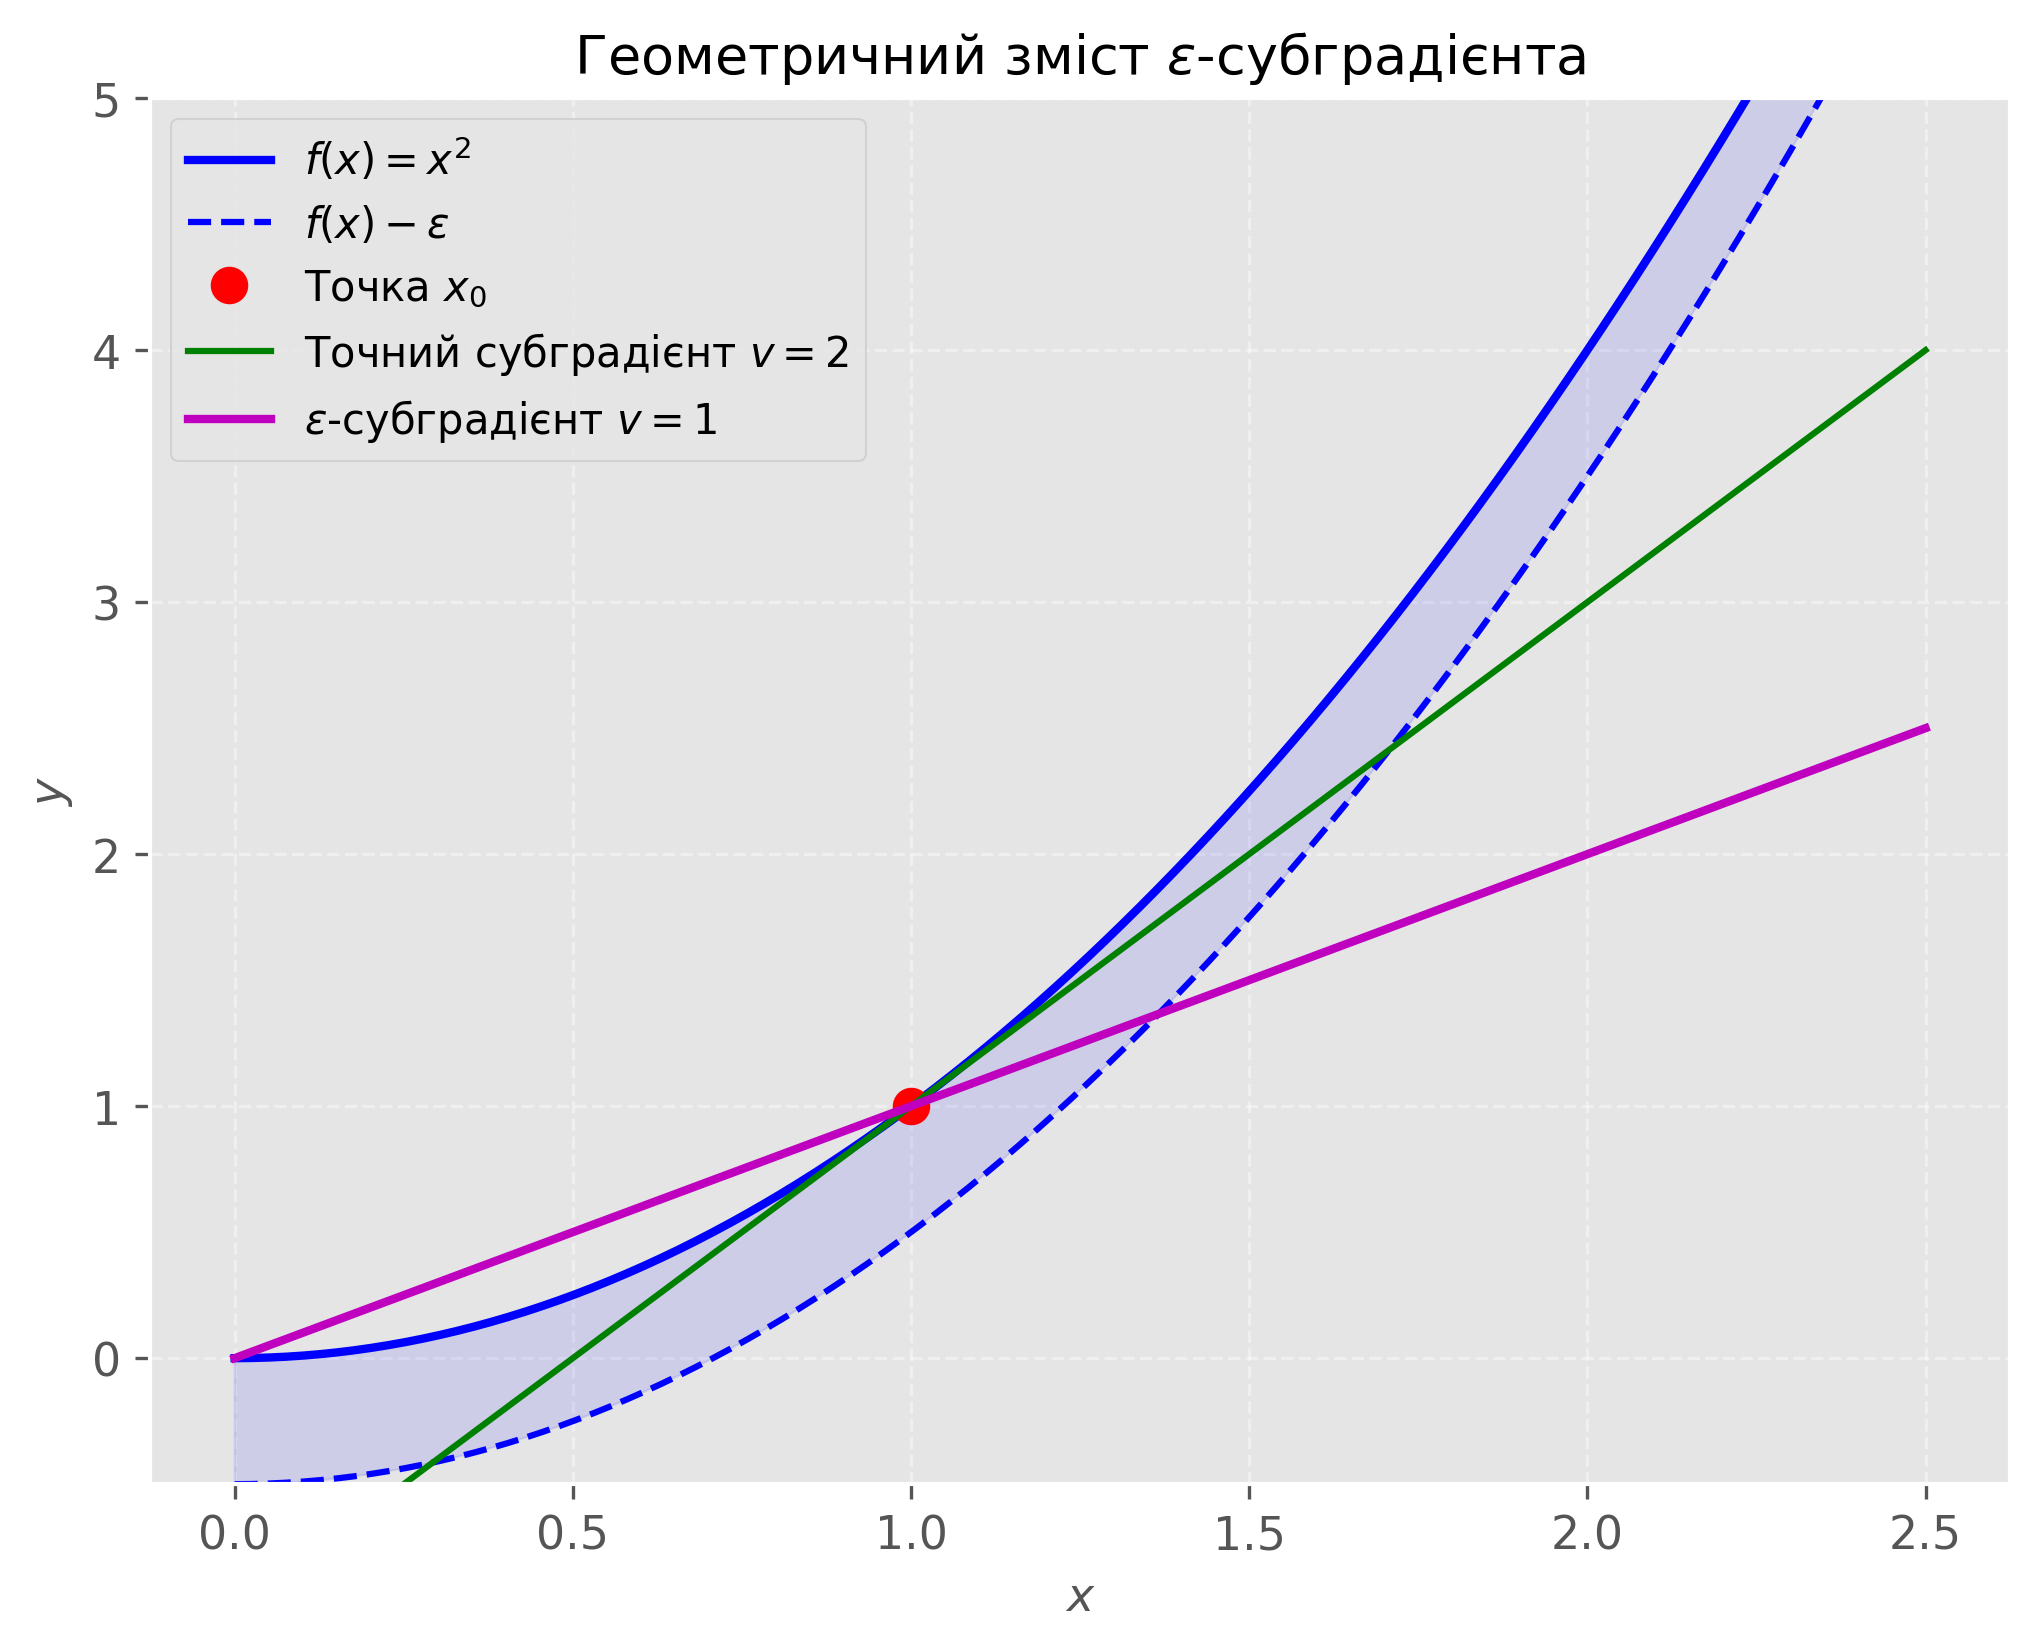
\includegraphics[width=0.85\textwidth]{eps_subgradient.png}
\caption{Геометрія $\varepsilon$-субградієнта: вектор $v=1$ не є дотичною, але утримує функцію в межах похибки $\varepsilon$.}
\label{fig:eps-subgradient}
\end{figure}

На кожному кроці $\varepsilon$-субградієнтний метод обчислює елемент мінімальної норми з наближеного субдиференціала:
$$
v_k = \arg\min_{v \in \partial_{\varepsilon_k} f(x_k)} \|v\|.
$$
Напрямок руху вибирається як $g_k = -v_k$. При цьому параметр $\varepsilon_k \downarrow 0$ монотонно зменшується з ростом ітерацій.

\section{Напрямок найкрутішого спуску за Кларком.}
Для мінімізації негладких, але локально ліпшицевих (не обов'язково опуклих) функцій напрямок найшвидшого локального спадання визначається через проекцію нуля на субдиференціал Кларка.

Напрямок $g_k$ знаходять як розв'язок задачі:
$$
z_k = \arg\min_{z \in \partial_C f(x_k)} \|z\|.
$$
Якщо $z_k = 0$, то поточна точка є стаціонарною за Кларком, і алгоритм завершує роботу. Інакше напрямок найкрутішого спуску задається вектором:
$$
g_k = -\frac{z_k}{\|z_k\|}.
$$

\begin{figure}[htbp]
\centering
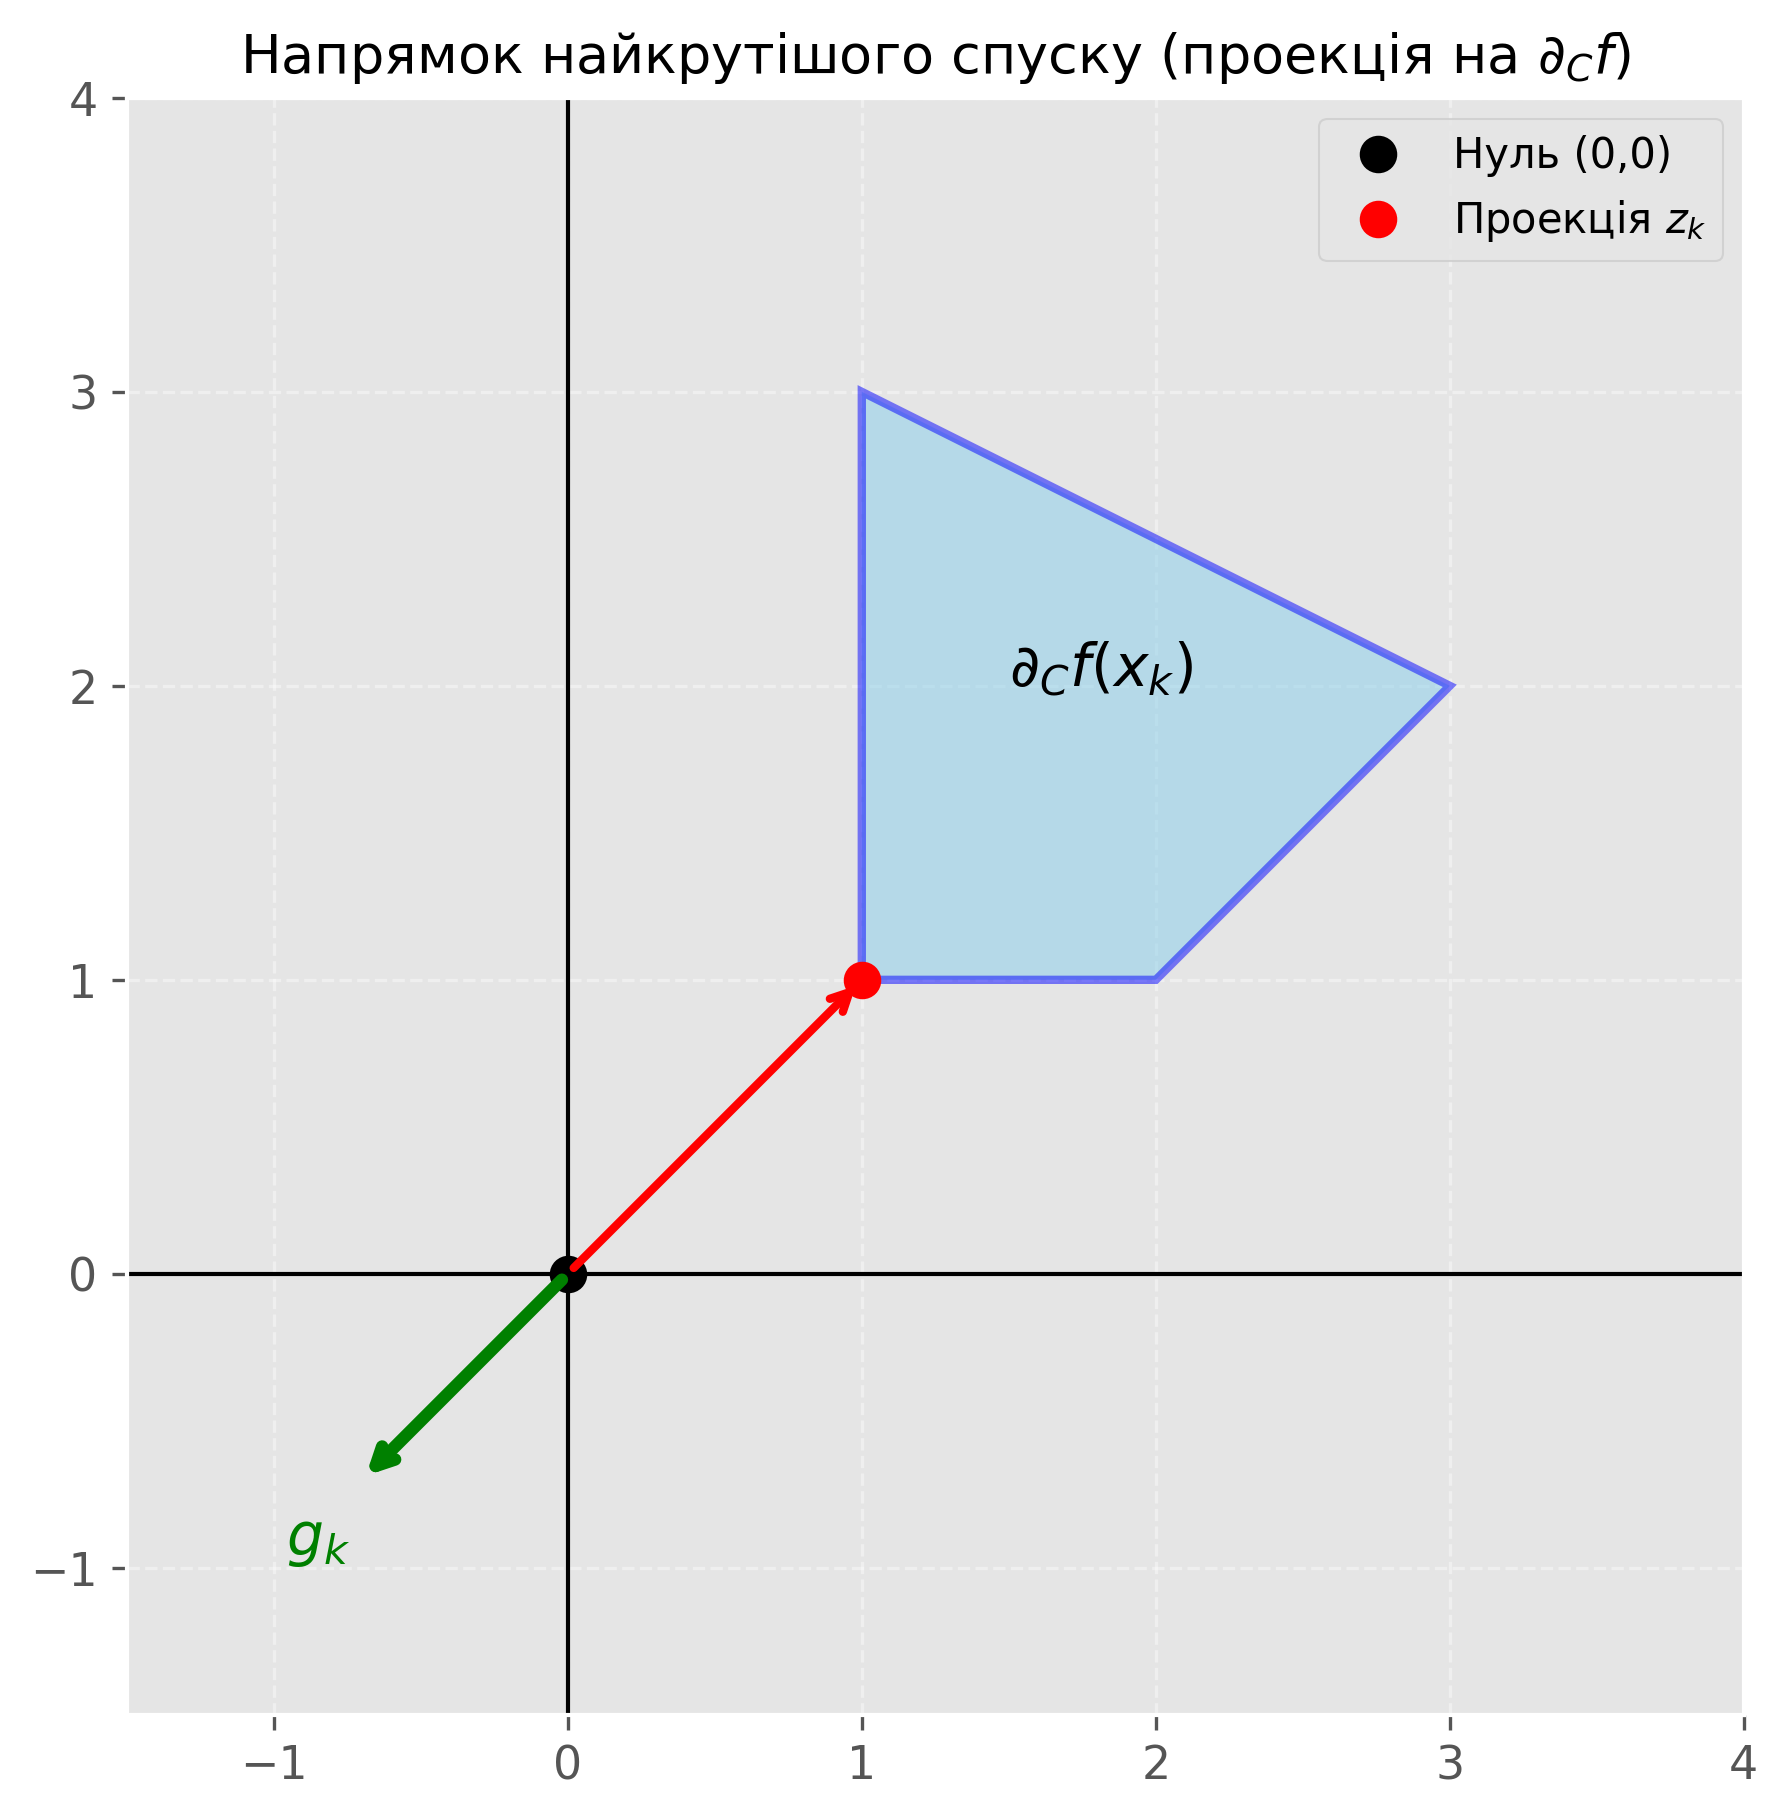
\includegraphics[width=0.75\textwidth]{clarke_descent.png}
\caption{Визначення напрямку найкрутішого спуску $g_k$ як антипода до проекції нуля $z_k$ на множину субдиференціала Кларка $\partial_C f(x_k)$.}
\label{fig:clarke-descent}
\end{figure}

\section{Метод узагальненого градієнтного спуску (МУГС Шора).}
Для мінімізації негладких опуклих функцій звичайний градієнтний спуск не застосовується, бо антисубградієнт не обов'язково є напрямком спуску. Н.~З.~Шор запропонував метод крокування з нормуванням кроку.

Ітераційна процедура має вигляд:
$$
x_{k+1} = x_k - \alpha_k \frac{v_k}{\|v_k\|}, \quad v_k \in \partial f(x_k).
$$
Для гарантії збіжності до глобального мінімуму параметри кроку $\alpha_k > 0$ повинні задовольняти умови розбіжного ряду з прямуванням до нуля:
$$
\lim_{k \to \infty} \alpha_k = 0, \quad \sum_{k=0}^{\infty} \alpha_k = \infty.
$$
Типовий вибір кроку: $\alpha_k = \frac{c}{k}$ або $\alpha_k = \frac{c}{\sqrt{k}}$.

\section{Метод узагальненого субградієнтного спуску В.~Ф.~Дем'янова.}
Цей метод використовує конструкцію $\mu$-субдиференціала для локального пошуку оптимуму.

Фіксують $\mu > 0$ і розглядають елементи $\omega = (s, w) \in d_{\mu}f(x)$, де $0 \leq s \leq \mu$, $w \in \mathbb{R}^n$. Для кожного $\omega$ будується лінійний підпростір (зміщений субдиференціал):
$$
L_{\omega}(x_k) = \partial f(x_k) + \omega.
$$
Для кожного $\omega \in d_{\mu}f(x_k)$ обчислюють вектор мінімальної норми:
$$
z_k^{\omega} = \arg\min_{z \in L_{\omega}(x_k)} \|z\|.
$$

\begin{figure}[htbp]
\centering
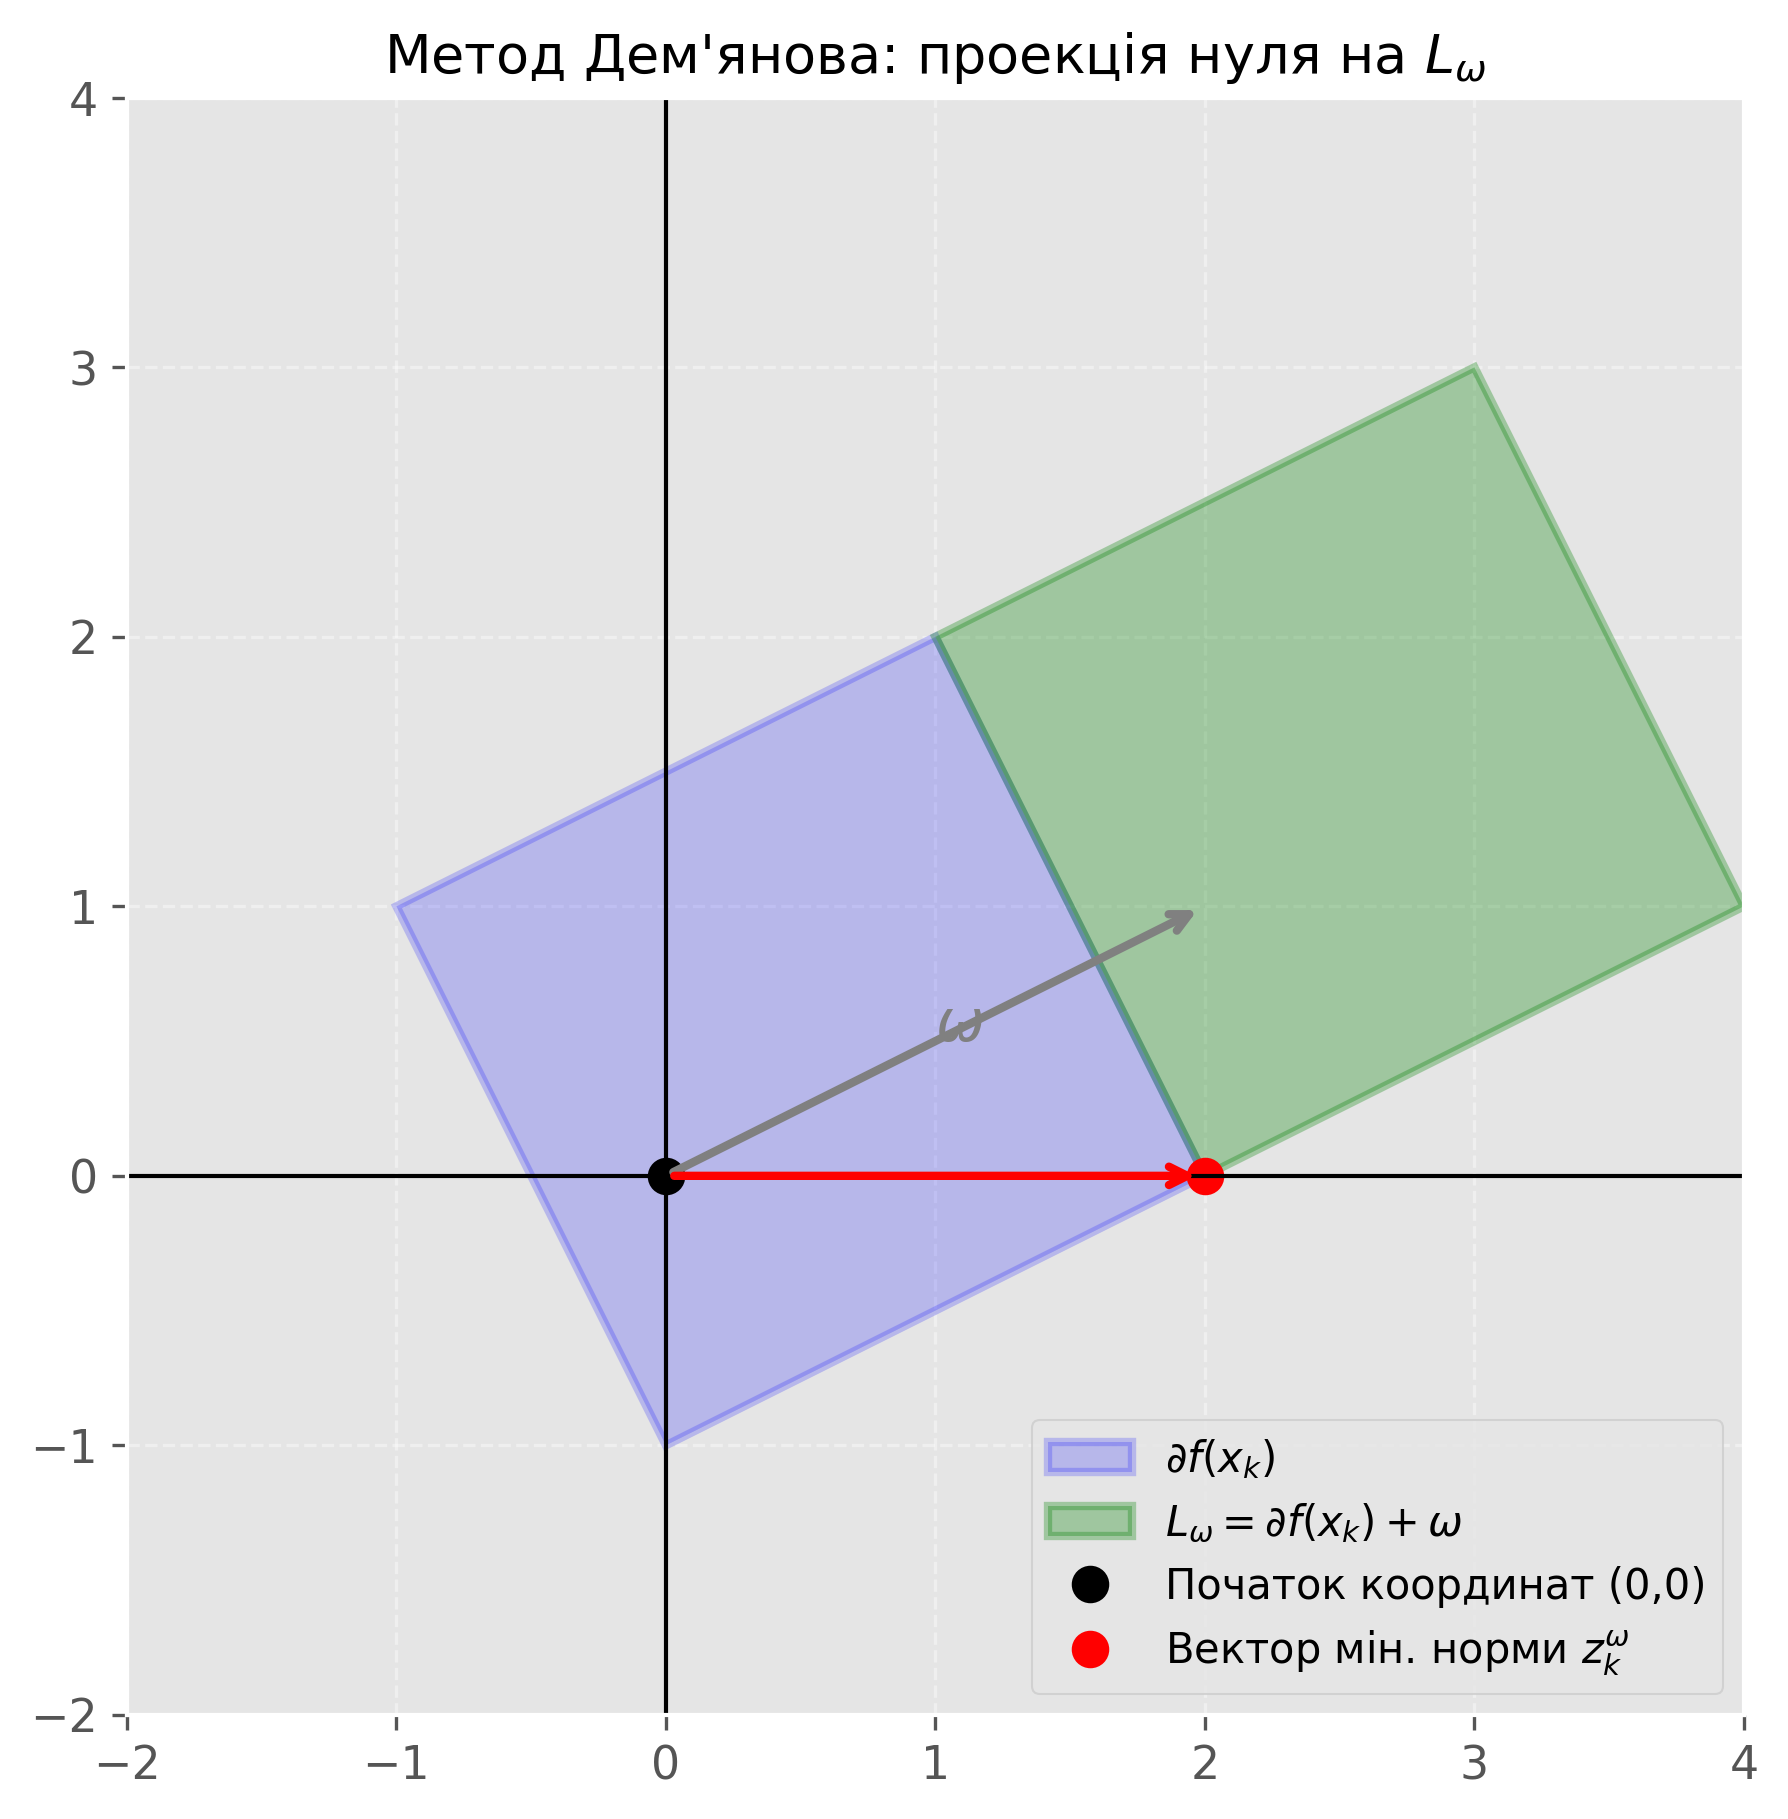
\includegraphics[width=0.75\textwidth]{demyanov_shift.png}
\caption{Крок методу Дем'янова: базовий субдиференціал зсувається на вектор $\omega$, утворюючи множину $L_\omega$, на якій відшукується елемент із мінімальною евклідовою нормою.}
\label{fig:demyanov-shift}
\end{figure}

Оптимальний напрямок спуску, що відповідає даному $\omega$, має вигляд $g_{\omega}(x_k) = -\frac{z_k^{\omega}}{\|z_k^{\omega}\|}$.

Далі виконується одновимірна мінімізація вздовж променя для кожного можливого напрямку:
$$
\min_{\alpha > 0} f(x_k - \alpha z_k^{\omega}) = f(x_k - \alpha_k^{\omega} z_k^{\omega}).
$$
На фінальному етапі кроку здійснюється дискретна мінімізація за всіма параметрами $\omega$, обираючи найкращий вектор $\omega_k$:
$$
\min_{\omega \in d_{\mu}f(x_k)} f(x_k - \alpha_k^{\omega} z_k^{\omega}) = f(x_k - \alpha_k^{\omega_k} z_k^{\omega_k}).
$$
Наступна ітерація: $x_{k+1} = x_k - \alpha_k^{\omega_k} z_k^{\omega_k}$.

\part{Конуси та двоїстість}

\section{Дотичний конус Булігана та конус можливих напрямків.}
Для моделювання локальної структури допустимих множин у задачах з обмеженнями використовуються конічні апроксимації.

\textbf{Означення.} \textit{Дотичним конусом Булігана} до множини $X \subset \mathbb{R}^n$ у точці $x \in X$ називають множину:
$$
T(X, x) = \left\{ g \in \mathbb{R}^n \mid \exists \{x_k\} \subset X,\, x_k \to x,\, \exists \{\lambda_k\} > 0 : \lim_{k \to \infty} \lambda_k(x_k - x) = g \right\}.
$$

\textbf{Означення.} \textit{Конусом можливих напрямків} до множини $X$ у точці $x \in X$ називають множину:
$$
P(X, x) = \{ g \in \mathbb{R}^n \mid \exists \alpha_0 > 0 : x + \alpha g \in X \quad \forall \alpha \in [0, \alpha_0] \}.
$$
Для довільної множини має місце включення $\overline{P}(X, x) \subset T(X, x)$. Якщо множина $X$ опукла, то їхні замикання збігаються: $\overline{P}(X, x) = T(X, x)$.

\begin{figure}[htbp]
\centering
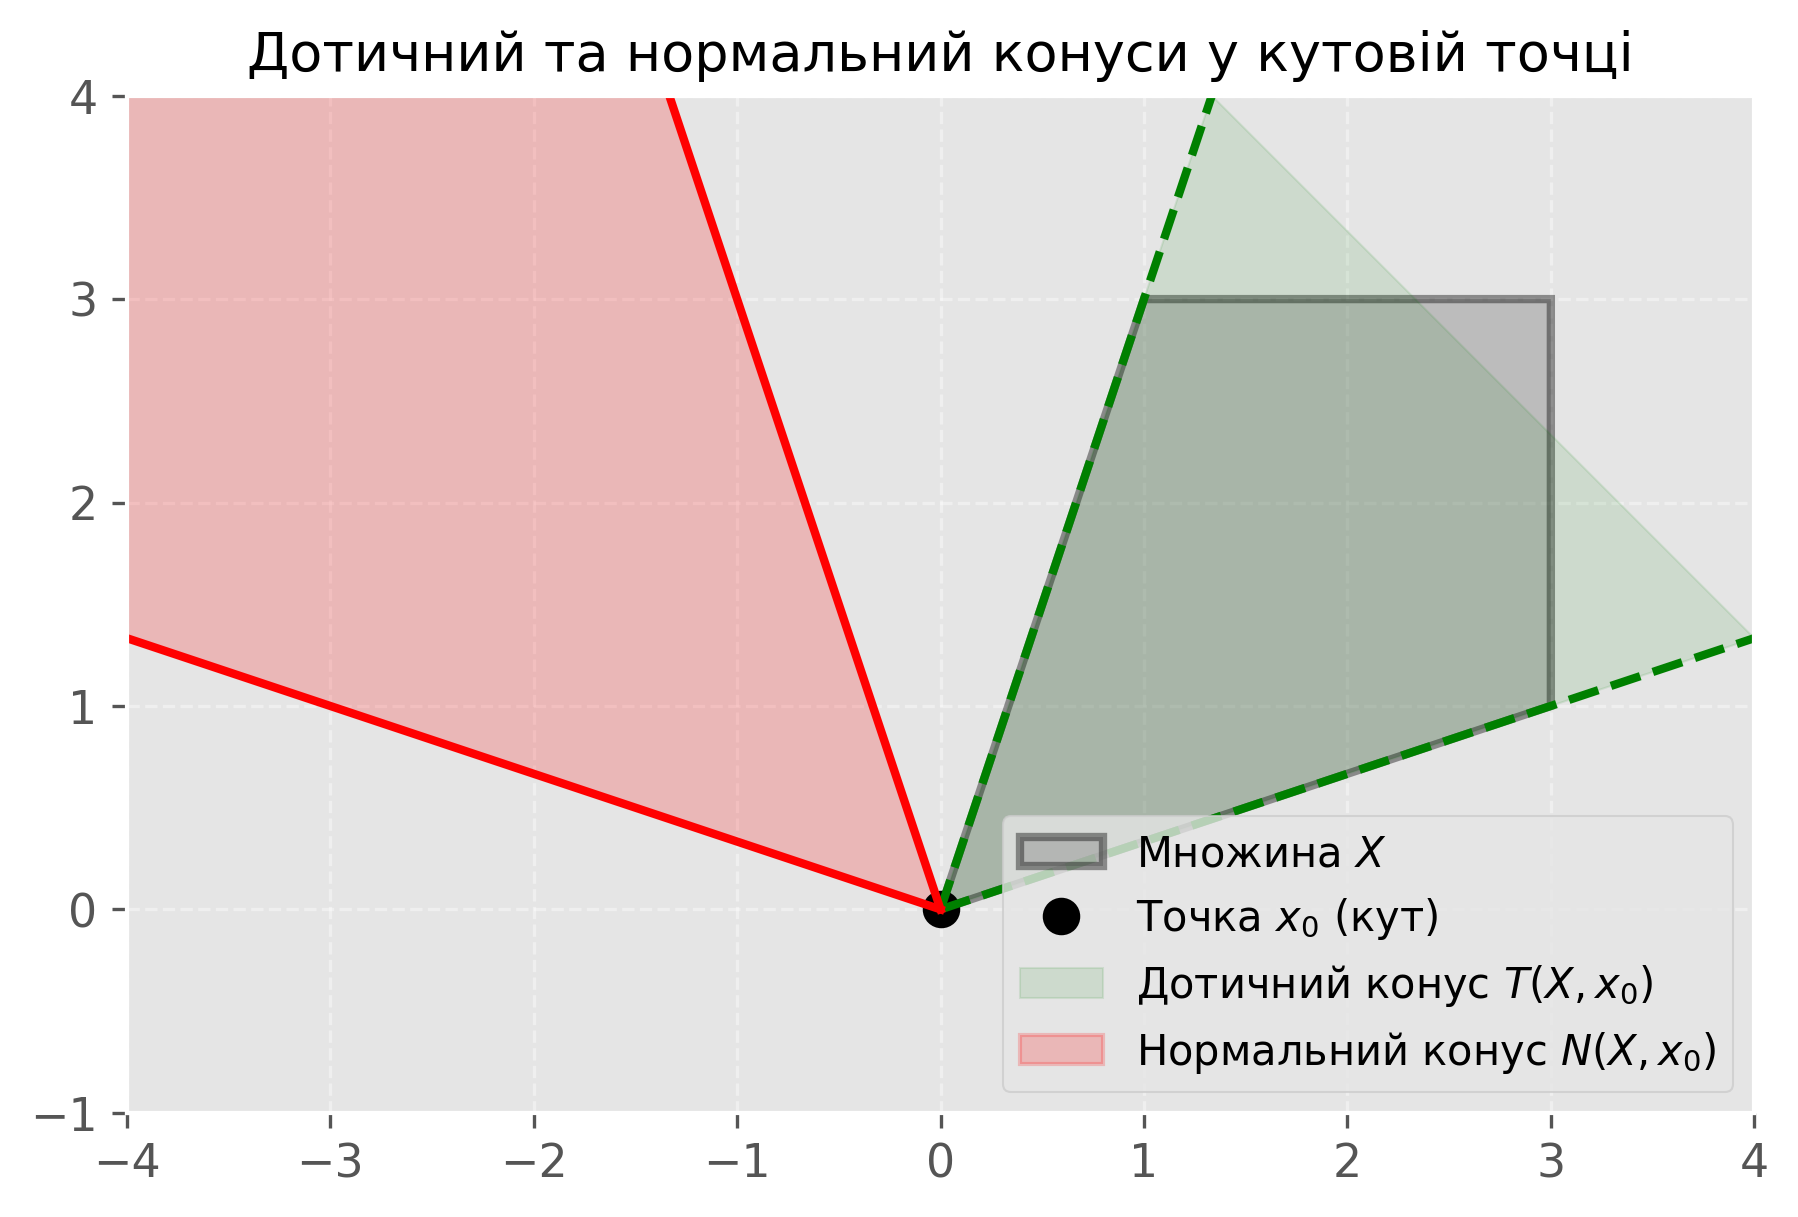
\includegraphics[width=0.7\textwidth]{bouligand_cones.png}
\caption{Дотичний конус розширює «кут» множини назовні, а нормальний конус є його полярою --- множиною всіх векторів, що утворюють тупий кут із дотичними напрямками.}
\label{fig:bouligand-cones}
\end{figure}

\section{Нормальний конус.}
\textbf{Означення.} \textit{Нормальним конусом} $N(X, x)$ до множини $X$ у точці $x \in X$ називають полярою (негативний спряжений конус) до дотичного конуса Булігана:
$$
N(X, x) = \{ v \in \mathbb{R}^n \mid \langle v, g \rangle \leq 0 \quad \forall g \in T(X, x) \}.
$$

Якщо множина $X$ опукла, то означення спрощується до класичного опорного вигляду:
$$
N(X, x) = \{ v \in \mathbb{R}^n \mid \langle v, y - x \rangle \leq 0 \quad \forall y \in X \}.
$$

\section{Функція Лагранжа.}
Розглянемо задачу опуклого програмування з обмеженнями-нерівностями:
$$
f_0(x) \to \min, \quad S = \{ x \in X \mid f_i(x) \leq 0,\,\, і = 1, \dots, m \},
$$
де $X \subset \mathbb{R}^n$ --- опукла множина, а $f_0, f_i$ --- опуклі $f_0, f_i$ є опуклими.

\textbf{Означення.} \textit{Функцією Лагранжа} цієї задачі називають функцію $L: X \times \mathbb{R}_+^m \to \mathbb{R}$, що визначається як:
$$
L(x, \lambda) = f_0(x) + \sum_{i=1}^m \lambda_i f_i(x),
$$
де $\lambda = (\lambda_1, \dots, \lambda_m)^T \geq 0$ --- вектор множників Лагранжа.

\section{Умова Слейтера та теорема Куна-Таккера.}
Для того, щоб умови оптимізації через функцію Лагранжа були двоїсто еквівалентними, необхідна регулярність обмежень.

\textbf{Умова регулярності Слейтера.} Для задачі опуклого програмування виконується умова Слейтера, якщо існує така точка $x_0 \in \operatorname{ri} X$, у якій всі обмеження-нерівності виконуються строго:
$$
f_i(x_0) < 0 \quad \forall і = 1, \dots, m.
$$

\textbf{Теорема (Куна-Таккера в диференційній формі).} Нехай для опуклої задачі виконується умова Слейтера. Точка $x^* \in S$ є оптимальним розв'язком задачі тоді і тільки тоді, коли існує такий вектор множників Лагранжа $\lambda^* = (\lambda^*_1, \dots, \lambda^*_m)^T \geq 0$, що виконуються дві умови:
\begin{enumerate}
    \item Стаціонарність функції Лагранжа по $x$:
    $$
    0 \in \partial_x L(x^*, \lambda^*) = \partial f_0(x^*) + \sum_{i=1}^m \lambda^*_i \partial f_i(x^*).
    $$
    \item Умова доповнюючої нежорсткості:
    $$
    \lambda^*_i f_i(x^*) = 0 \quad \forall і = 1, \dots, m.
    $$
\end{enumerate}


% =========================================================================
% МЕТОДИ НЕГЛАДКОЇ ОПТИМІЗАЦІЇ
% =========================================================================

\part{Напрямлене диференціювання та числення Кларка}

\section{Локально ліпшицева функція.}
У негладкому аналізі для функцій, які не є опуклими, базовим класом регулярності є локальна ліпшицевість, яка замінює вимогу неперервної диференційовності.

\textbf{Означення.} Функцію $f: \mathbb{R}^n \to \mathbb{R}$ називають \textit{локально ліпшицевою} в околі точки $x_0 \in \mathbb{R}^n$, якщо існують такі додатні сталі $L > 0$ (стала Ліпшиця) та $\varepsilon > 0$, що для будь-яких двох точок $x_1, x_2 \in B(x_0, \varepsilon)$ виконується нерівність:
$$
|f(x_1) - f(x_2)| \leq L \|x_1 - x_2\|.
$$

За теоремою Радемахера локально ліпшицева функція диференційовна майже скрізь (за мірою Лебега).

\section{Узагальнена похідна Кларка за напрямком.}
Для локально ліпшицевих функцій класична границя відношення приросту може не існувати. Ф.~Кларк запропонував регулярну регуляризацію через верхню границю за двома змінними.

\textbf{Означення.} \textit{Узагальненою похідною Кларка за напрямком} $g \in \mathbb{R}^n$ локально ліпшицевої функції $f$ у точці $x$ називають величину:
$$
f^{\circ}(x; g) = \limsup_{\substack{y \to x \\ t \downarrow 0}} \frac{f(y + tg) - f(y)}{t},
$$
де $y \in \mathbb{R}^n$, а $t$ прямує до нуля, залишаючись додатним ($t > 0$).

Для локально ліпшицевої $f$ величина $f^{\circ}(x; g)$ скінченна, $|f^{\circ}(x; g)| \leq L\|g\|$, субадитивна та додатньо однорідна за $g$.

\section{Субдиференціал Кларка.}
\textbf{Означення.} \textit{Субдиференціалом Кларка} локально ліпшицевої функції $f$ у точці $x$ називають множину $\partial_C f(x) \subset \mathbb{R}^n$, яка визначається як геометричний субдиференціал сублінійної функції $g \to f^{\circ}(x; g)$:
$$
\partial_C f(x) = \{ v \in \mathbb{R}^n \mid \langle v, g \rangle \leq f^{\circ}(x; g) \quad \forall g \in \mathbb{R}^n \}.
$$

\textbf{Властивості субдиференціала Кларка:}
\begin{enumerate}
    \item $\partial_C f(x)$ є непорожньою, опуклою та компактною множиною в $\mathbb{R}^n$.
    \item Якщо $f$ є опуклою функцією, то її субдиференціал Кларка повністю збігається із класичним субдиференціалом опуклого аналізу.
    \item Якщо $f$ є неперервно диференційовною в околі точки $x$, то субдиференціал Кларка складається з одного вектора --- градієнта: $\partial_C f(x) = \{ \nabla f(x) \}$.
\end{enumerate}

\section{Необхідна умова екстремуму за Кларком.}
\textbf{Теорема (Необхідна умова локального екстремуму).} Якщо точка $x^* \in \mathbb{R}^n$ є точкою локального мінімуму або локального максимуму локально ліпшицевої функції $f(x)$, то нульовий вектор належить її субдиференціалу Кларка:
$$
0 \in \partial_C f(x^*).
$$
Точки, які задовольняють цю умову, називаються \textit{стаціонарними за Кларком}.


% =========================================================================
% КОНУСИ ТА ДВОЇСТІСТЬ
% =========================================================================

\part*{Література}
\addcontentsline{toc}{part}{\numberline{}Література}

\noindent\hangindent=1.25cm\hangafter=1
1. Моклячук М.~П. \emph{Негладкий аналіз та оптимізація}~: навч. посіб. / М.~П.~Моклячук.~--- К.~: ВПЦ <<Київський університет>>, 2008.~--- 384~с.


\end{document}
